\section{Scoliosi (trattamento)}

\emph{La parte più consistente dell'epidemiologia è rappresentata dalle scoliosi infantili idiopatiche che sono le più frequenti e sono quelle che traggono più in inganno perché sono moltissime, ma in realtà quelle che vanno curate sono pochissime. Il problema quindi è riconoscere quelle che richiedono effettivamente un trattamento.}

Vi ricordo che c'è un rapporto tra peggioramento attivo e età scheletrica: una bambina di 14-15 anni già sviluppata da due anni, probabilmente, non dovendo più crescere, non ha più la possibilità di
avere un peggioramento di tipo attivo.

Nella lezione precedente abbiamo visto anche il peggioramento passivo che però è percentualmente molto inferiore rispetto a quello che è il peggioramento attivo durante il periodo dell'accrescimento.

\begin{figure}[!ht]
\centering
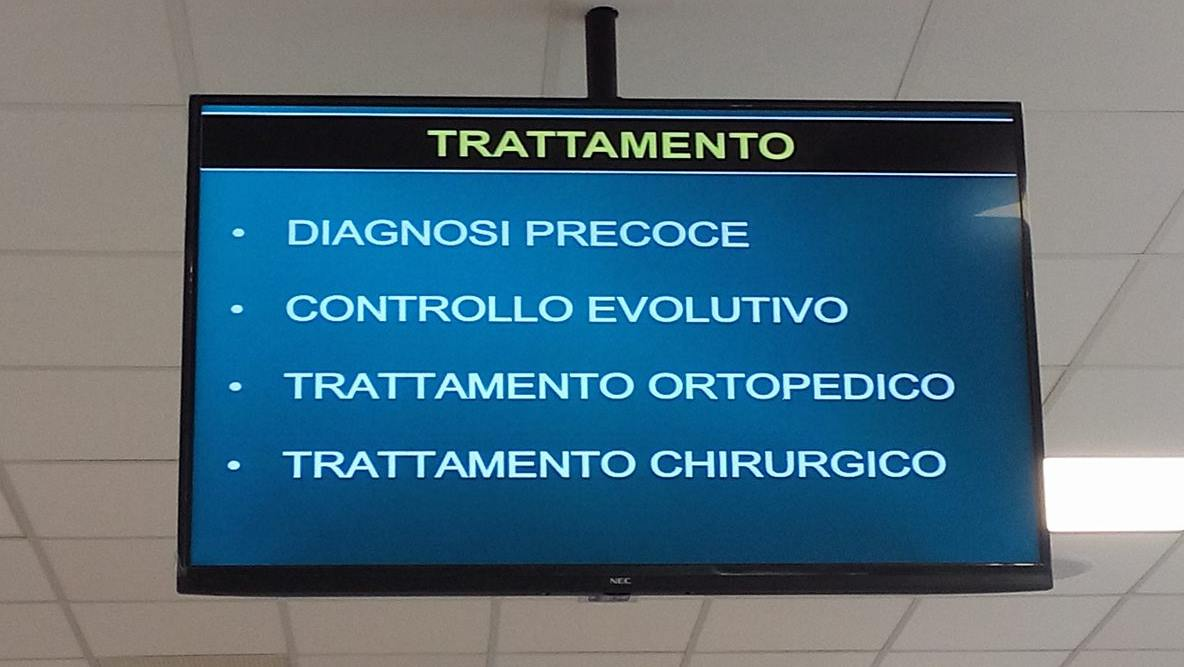
\includegraphics[width=0.4\textwidth]{013/image1.jpeg}
\end{figure}

Vi ricordo che non esiste prevenzione per la scoliosi \emph{e questo confuta tutto quanto comunemente si crede circa la possibilità di prevenire il peggioramento della stessa con la ginnastica correttiva, il nuoto, dormendo su un letto rigido oppure con terapie come l'elettrostimolazione della muscolatura della convessità della curva.}

Il trattamento dello scoliosi può essere così schematizzato:

\begin{itemize}
\item
  \textbf{Diagnosi precoce}
\item
  \textbf{Controllo evolutivo}
\item
  \textbf{Trattamento ortopedico}
\item
  \textbf{Trattamento chirurgico (eventualmente)}
\end{itemize}

\subsection{Diagnosi precoce}

\emph{Questa è l'unica terapia utile! Non significa solo individuare la curva e riconoscere sia una scoliosi vera o organica (questa fase potrebbe essere anche relativamente agevole) piuttosto \textbf{\emph{capire quella scoliosi}} e \textbf{\emph{valutare se necessiti di un trattamento o meno}}. Possono infatti presentarsi due evenienze:}

\begin{itemize}
\item
  \emph{La \emph{gravità} della scoliosi è \emph{modesta} per cui sarà fondamentale il \emph{controllo evolutivo} in relazione all'accrescimento. Questo sarà realizzato tramite controlli periodici e solo \emph{eventualmente} si ricorrerà alla terapia ortopedica e/o chirurgica}
\item
  \emph{La \emph{scoliosi} si presenta \emph{già in una forma severa}
  \emph{o} comunque \emph{significativa} così da imporre fin da subito la necessità di un trattamento ortopedico e/o chirurgico \emph{anche se lo sviluppo e la fase di accrescimento non si sono ancora concluse}}
\end{itemize}

\subsection{Controllo evolutivo}

\emph{Durante una visita ortopedica si valutano i fattori di tipizzazione all'Rx} (\emph{vedere sbobina precedente sulle scoliosi per i fattori di tipizzazione}). \emph{Se il bambino ha una \textbf{\emph{lieve scoliosi}} ed è \textbf{\emph{in età di accrescimento}}, si fa un controllo dopo 6-8 mesi per stimare il rapporto tra eventuale accrescimento (si misura l'altezza) e peggioramento (si chiede una radiografia). Se la scoliosi è rimasta invariata allora la bambina o il bambino tornano a casa e continuano la loro vita normale. \emph{Si procederà con questi controlli periodici fino al termine della fase di accrescimento che è il periodo critico}. Il prof parla di \textbf{Energica Terapia di Attesa} (IMPARARE QUESTA ESPRESSIONE!).} Se invece la scoliosi è importante già alla prima visita, si procede con il trattamento ortopedico e/o chirurgico anche se lo sviluppo non è completato.

Il concetto fondamentale \textbf{\emph{non è quello di curare le scoliosi tutte e subito}}, ma di \textbf{\emph{capirle}}: dobbiamo capire se è

\begin{itemize}
\item
  Una di quelle poche che \emph{così sono e così rimarranno} e che sono di circa 8 gradi in un adulto (curva non perfetta, ma normale)
\item
  Una \textbf{forma evolutiva} che nella fase successiva \emph{andrà incontro a peggioramento.} In questo ultimo caso bisogna cercare di \emph{\emph{bloccare o limitare il peggioramento sfruttando se possibile l'accrescimento e quindi la possibilità di un miglioramento.}}
\end{itemize}

Il primo obiettivo quindi non è mai quello di raddrizzare la colonna bensì di \textbf{bloccare un eventuale peggioramento}: su 100 scoliosi che vediamo in 3-4 c'è rischio di peggioramento e quindi la necessità di
mettere dei busti o fare trattamenti. Invece le altre si accompagnano e seguono fino alla fine del periodo ``pericoloso'' dell'accrescimento attraverso controlli periodici e ne residueranno delle scoliosi sì, ma
modeste e assolutamente compatibili con una buona qualità di vita.
{[}\emph{Il prof si sofferma particolarmente su questo aspetto anche in relazione alle conseguenze negative cui il paziente andrà in corso in caso di errata interpretazione della forma di scoliosi. Inoltre ricorda che il danno medico non consiste solo nel danno organico, ma c'è anche un danno di tipo \emph{diagnostico-evolutivo} nel momento in cui non si comprende quel tipo di scoliosi. {]}}
\\\\
Quindi si curano solo quelle peggiorano? \textbf{\emph{In parte sì}}!
Può anche capitare di vedere \textbf{\emph{una bambina di 10 anni già con una curva di moderata gravità (15-20 gradi). Anche se si deve ancora sviluppare comunque ha già una scoliosi importante quindi facciamo subito un trattamento ortopedico con corsetto o un trattamento chirurgico.}} In entrambi gli approcci \emph{l'accrescimento diventa un alleato utile} nella terapia. È facile quindi in questo campo fare la diagnosi, ma i problemi sorgono poi quando si tratta di fare il trattamento. Le variabili in campo sono tantissime e vanno considerate tutte insieme in modo tale da tirar fuori una valutazione, mediata anche dall'esperienza, che porti poi a fare trattamento o meno evitando indicazioni inutili come il nuoto, la ginnastica correttiva, il materasso duro (che male non fanno, ma fanno perdere tempo e in qualche caso a distanza di 2-3 anni si vedono colonne che peggiorano e devono essere operate). \emph{Queste indicazioni non hanno alcun valore né sull'innesco, né sulla prevenzione della scoliosi, né sulla prevenzione del peggioramento. }

Un tentativo terapeutico proposto, ma che non ha avuto alcun successo, consiste nello stimolare i muscoli che sono dalla parte della convessità della curva: si parte dal presupposto che i muscoli della concavità tirino di più, mentre quelli della convessità tirino di meno. Si pensò
così di fare delle elettrostimolazioni sui muscoli che sostengono la colonna dalla parte dove sono più sgonfi. In realtà il risultato è stato deludente.

Ricapitolando: punto imprescindibile è una \textbf{\emph{precoce diagnosi}} e una \textbf{\emph{corretta}} \textbf{\emph{valutazione}}
del tipo di scoliosi \textbf{\emph{così da trattare}} solo quelle che effettivamente lo richiedono:

\begin{itemize}
\item
  Scoliosi per le quali esiste un \textbf{\emph{rischio accertato di aggravamento}}
\item
  Scoliosi in cui \textbf{\emph{già alla prima osservazione si abbiano gradi elevati di curvatura}} anche se lo sviluppo non fosse ancora completato (tipo di 30 gradi)
\end{itemize}

\subsection{Trattamento ortopedico}
Questo consiste prevalentemente nell'utilizzo dei corsetti o busti. Ce ne sono di diversi tipi e ogni scuola usa quelli che ritiene più giusti in base all'esperienza e alla filosofia di partenza. Normalmente i corsetti prendono il nome della città dove sono stati inventati.

Il corsetto deve:

\begin{itemize}
\item
  Essere fatto \emph{su misura} (non standard, ma individuale)
\item
  Essere \emph{rigido} altrimenti è il paziente che piega il busto e non è il busto che raddrizza il paziente
\item
  Avere delle sbarre di \emph{sostegno}, \emph{anelli cervicali, ecc}. (ci sono varie forme). Il corsetto agisce dall'esterno sulle principali deformazioni caratterizzanti la scoliosi ovvero il gibbo costale e la prominenza lombare: il pressore spinge sulle coste e le va a de-ruotare andando a de-ruotare ,attraverso le coste, anche le vertebre dorsali. Il meccanismo d'azione si basa su una \textbf{de-rotazione}, una \textbf{trazione} e una \textbf{spinta}
\item
  C'è una \textbf{fisiochinesiterapia} in corsetto ovvero guidata dal corsetto stesso
\item
  Avere una \emph{precocità}
\item
  Essere applicato \emph{in maniera esatta}
\item
  \emph{\emph{Va usato e usato correttamente (non basta comprarlo!)}}
\end{itemize}

\begin{figure}[!ht]
\centering
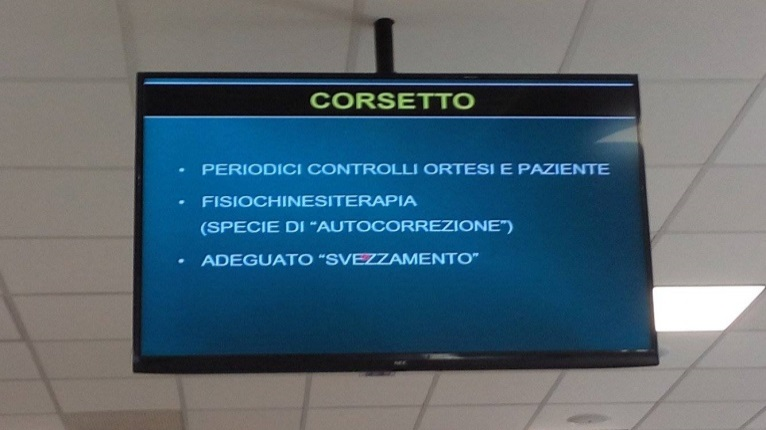
\includegraphics[width=0.4\textwidth]{013/image2.jpeg}
\end{figure}

Inoltre saranno necessari dei controlli periodici del paziente e dell'ortesi \emph{soprattutto nei bambini} che con il corsetto ci fanno di tutto perciò alla lunga questo può perdere di rigidità perché ad esempio si allentano le viti.

Inoltre si potrebbe osservare un \textbf{miglioramento} perciò la spinta iniziale data con il pressore può non essere più sufficiente dopo sei mesi. Ciò rende necessario aumentare tale spinta magari aumentando lo spessore del pressore.

Importanti sono:
\begin{itemize}
\item
  Lo \textbf{\emph{svezzamento}}: occorre un adeguato ``svezzamento'' dal corsetto cioè lo si porta fin quando non finisce l'accrescimento. Ad esempio lo mettiamo ad un bambino di 12 anni e questa lo porta per due anni fin quando non si osserva un miglioramento, a quel punto lo togliamo. Così facendo però sbaglieremmo perché il bambino non è ancora pienamente sviluppato \textbf{\emph{per cui con il successivo accrescimento perderemmo tutti i buoni risultati raggiunti}}. Quindi lo svezzamento \textbf{\emph{deve essere ragionato e graduale}} (es: portandolo solo la notte, ecc.)
\item
  \emph{La \textbf{correttezza e esattezza delle indicazioni}}: non bisogna mettere il corsetto a tutti i casi di scoliosi solo per ``avere la coscienza pulita''. Bisogna considerare che nell'adolescente non esiste solo l'implicazione organica, ma soprattutto quella \textbf{psicologica} per cui è importante individuare solo i casi in cui il trattamento è davvero necessario.
\end{itemize}

\begin{figure}[!ht]
\centering
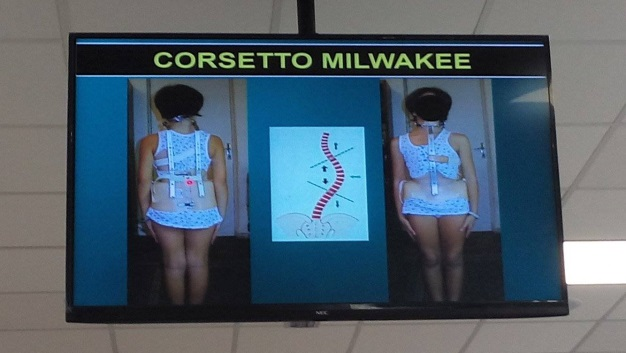
\includegraphics[width=0.4\textwidth]{013/image3.jpeg}
\end{figure}

Esempio di corsetto: a livello del gibbo toracico è posto un pressore e dall'altra parte agisce un pressore lombare fisso. Il corsetto esercita una trazione e delle pressioni sulle coste che permettono la de-rotazione della colonna.

Vediamo ora i vari tipo di corsetto:

\begin{itemize}
\item \textbf{Corsetto Milwakee,} \emph{ideale per le bambine piccole:
esercita una trazione del rachide, una pressione localizzata sulla convessità della curva e una pressione nella cintura pelvica a livello lombare (teoria dei tre punti). In una curva di scoliosi la parte interna della vertebra cresce meno perché sottoposta a maggiore pressione rispetto alla parte esterna perciò la colonna viene trazionata e spinta attraverso le coste in senso di de-rotazione, così che la deformità trapezoidale tenda a recuperare}.

\begin{figure}[!ht]
\centering
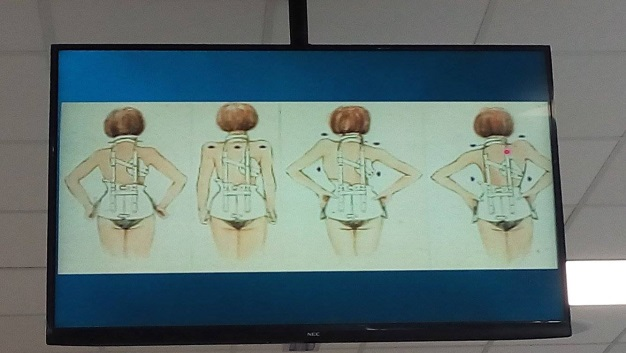
\includegraphics[width=0.4\textwidth]{013/image4.jpeg}
\end{figure}

Questi rappresentati sono esempi di esercizi in corsetto (di trazione, di allungamento, ma anche ad esempio alzare una spalla poi alzare l'altra e l'esercizio controlaterale) per cercare di ridurre queste curve.
Ultimamente questi esercizi sono stati però un po' superati.

\begin{figure}[!ht]
\centering
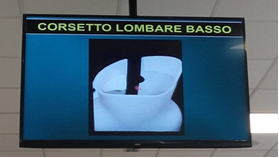
\includegraphics[width=0.4\textwidth]{013/image5.png}
\end{figure}

\item \textbf{Corsetto lombare basso (Bolognese)}, \emph{inventato a Bologna.}
\emph{È simile al corsetto Milwakee senza però un attacco superiore e serviva solo per le scoliosi lombari.}

\begin{figure}[!ht]
\centering
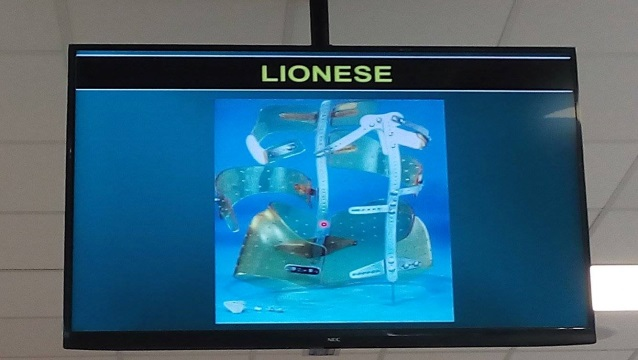
\includegraphics[width=0.4\textwidth]{013/image6.jpeg}
\end{figure}

\item \textbf{Corsetto Lionese,} \emph{si tratta di un corsetto molto più statico, ma che agisce come gli altri (con una pressione localizzata che determina la de-rotazione delle vertebre). Ideale per le ragazze già sviluppate perché più rigido e correttivo.}
\end{itemize}

A seconda delle metodiche usate nelle diverse scuole e della gravità della patologia, il corsetto può essere utilizzato:

\begin{itemize}
\item
  Solo di notte
\item
  Part-time (con 6-8 ore libere dal corsetto da gestirsi a piacimento nella giornata)
\item
  Tempo pieno
\end{itemize}

Dipende dalle varie situazioni: in una bambina di 13 anni magari sviluppata già da due mesi (quindi abbiamo ancora un anno, un anno e mezzo per sfruttare l'accrescimento) si cercherà di ridurre il tempo di libertà perché farle portare il corsetto solo di notte sarebbe poco. In
questo caso dal momento che il trattamento si presuppone di massimo un anno/un anno e mezzo (perché già sviluppata) quindi breve, si applica il corsetto a tempo pieno.

Se invece la bambina ha 9/10 anni, c'è a disposizione più tempo per poterla trattare e allora si può decidere di utilizzare il corsetto part-time permettendo anche otto ore libere durante la giornata.

Se poi il busto ha migliorato la curva, si può aumentare il tempo di libertà ad esempio facendoglielo portare solo la notte.

\begin{figure}[!ht]
\centering
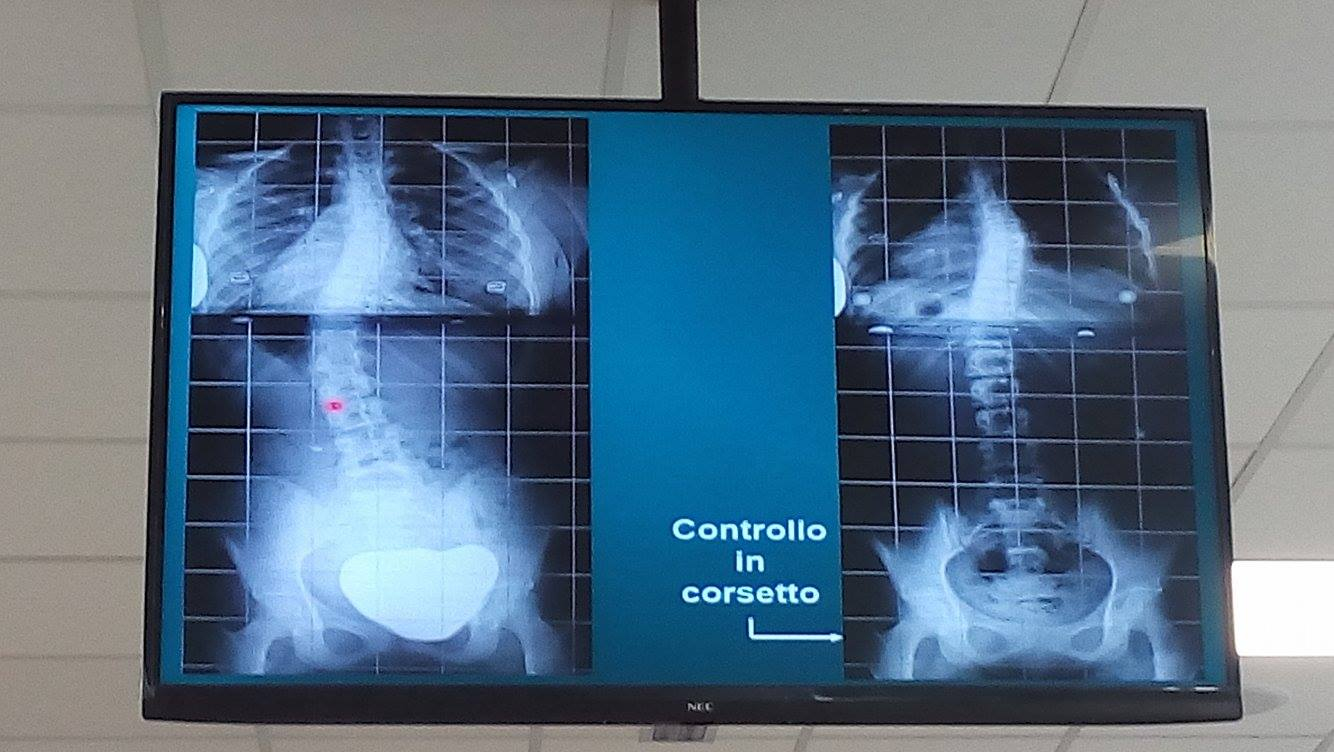
\includegraphics[width=0.4\textwidth]{013/image7.jpeg}
\end{figure}

Quella riportata è una classica radiografia dove si vede bene la curva: si tratta di una scoliosi vera. Di fianco la radiografia in corsetto per vedere se quel corsetto funziona o meno: non dobbiamo aspettarci di vedere una curva ``raddrizzata'' perché abbiamo a che fare con strutture che hanno una certa elasticità e più di tanto non si può fare.
Normalmente per vedere se quel corsetto lavora bene o no occorre studiare la plasticità dei dischi intervertebrali (trucco super specialistico): se un disco intervertebrale è ben ``aperto'' allora più di tanto non posso fare. Io posso agire spingendo solo sull'elasticità data dai dischi quindi non mi aspetterò in un simile caso di vedere una schiena dritta. C'è una certa elasticità che va rispettata.

Il trattamento non chirurgico può prevedere anche l'utilizzo dei gessi che ovviamente non potranno essere tolti. Il principio è lo stesso:
\emph{sfruttare meccanismi di pressione localizzata e trazione. Si mettono dei pressori che vengono poi ingessati nei busti. }

Vengono usati per esempio laddove il gibbo è molto accentuato oppure quando la scoliosi è più rigida e strutturata perché il corsetto di plastica lavora di più invece sulla parte estetica.

\begin{figure}[!ht]
\centering
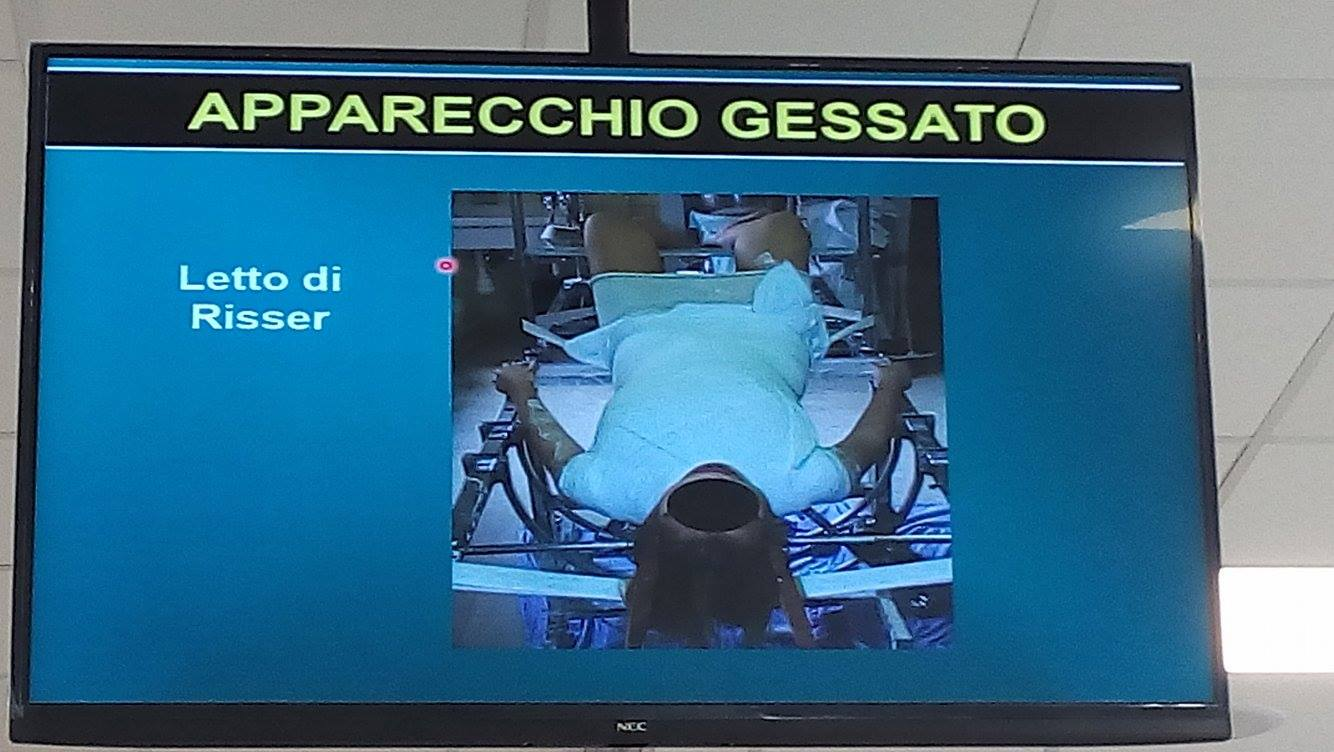
\includegraphics[width=0.4\textwidth]{013/image8.jpeg}
\end{figure}

Si controbilancia il fatto che non possano essere tolti facendone ad esempio tre in un inverno, di due mesi in due mesi, in modo tale da poter fare una doccia tra uno e l'altro. In estate solitamente non vengono fatti, se non nei casi più severi. È una correzione più statica
che si usa nei casi gravi.

\begin{figure}[!ht]
\centering
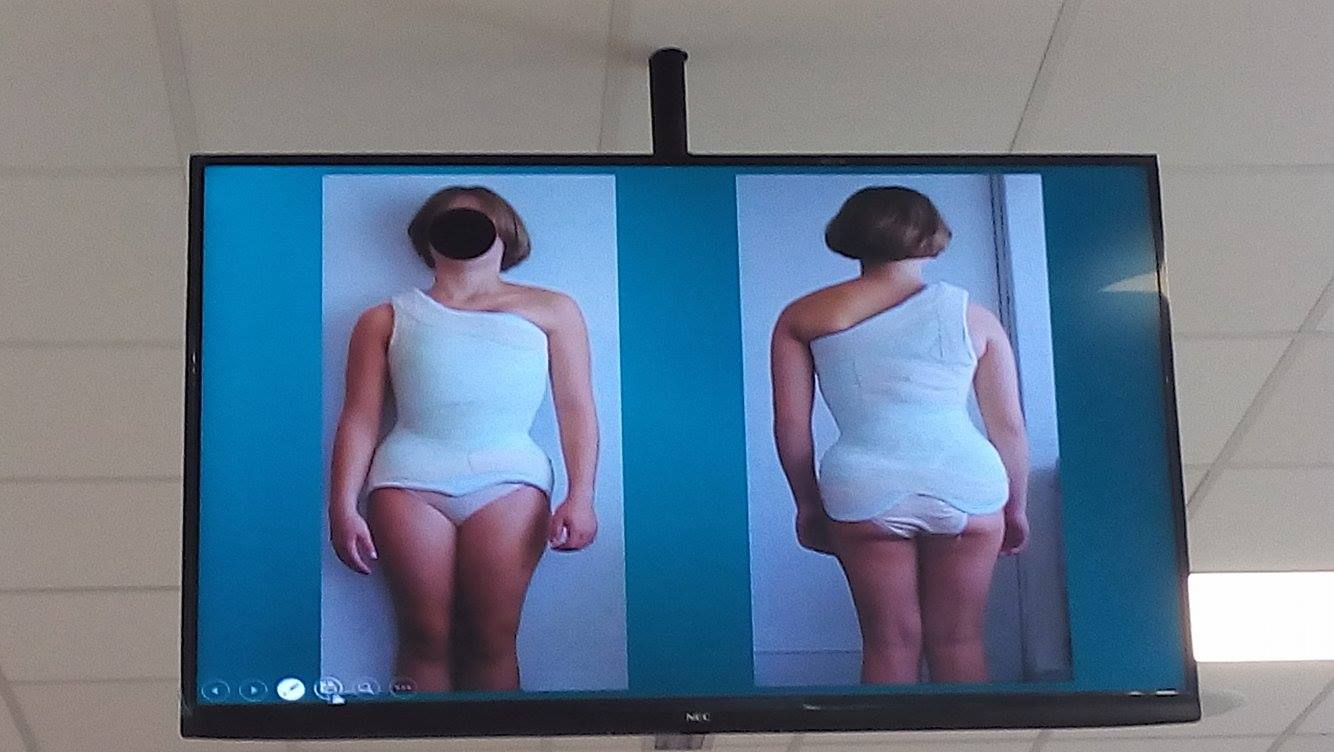
\includegraphics[width=0.4\textwidth]{013/image9.jpeg}
\end{figure}

Questi sono dei gessi la cui confezione è stata standardizzata a Pisa.

\subsection{Trattamento chirurgico}

Le indicazioni sono:

\begin{itemize}
\item
  Scoliosi grave, oltre i 40 gradi
\item
  Scoliosi di moderata entità in cui però il trattamento ortopedico sarebbe troppo lungo oppure se ci sono condizioni socio-economiche della famiglia per cui non si riesce a portare a termine il trattamento ortopedico (non fa portare il busto, non porta il bambino ai controlli) o un problema di mentalità per il quale non viene compresa la necessità del trattamento che quindi non viene effettuato.
\item
  Scoliosi in cui è fallito il trattamento ortopedico. Ci sono dei casi che in gergo si chiamano ``maligni'' in cui nonostante sia stato fatto tutto bene, c'è comunque un aggravamento della curva.
\end{itemize}

\begin{figure}[!ht]
\centering
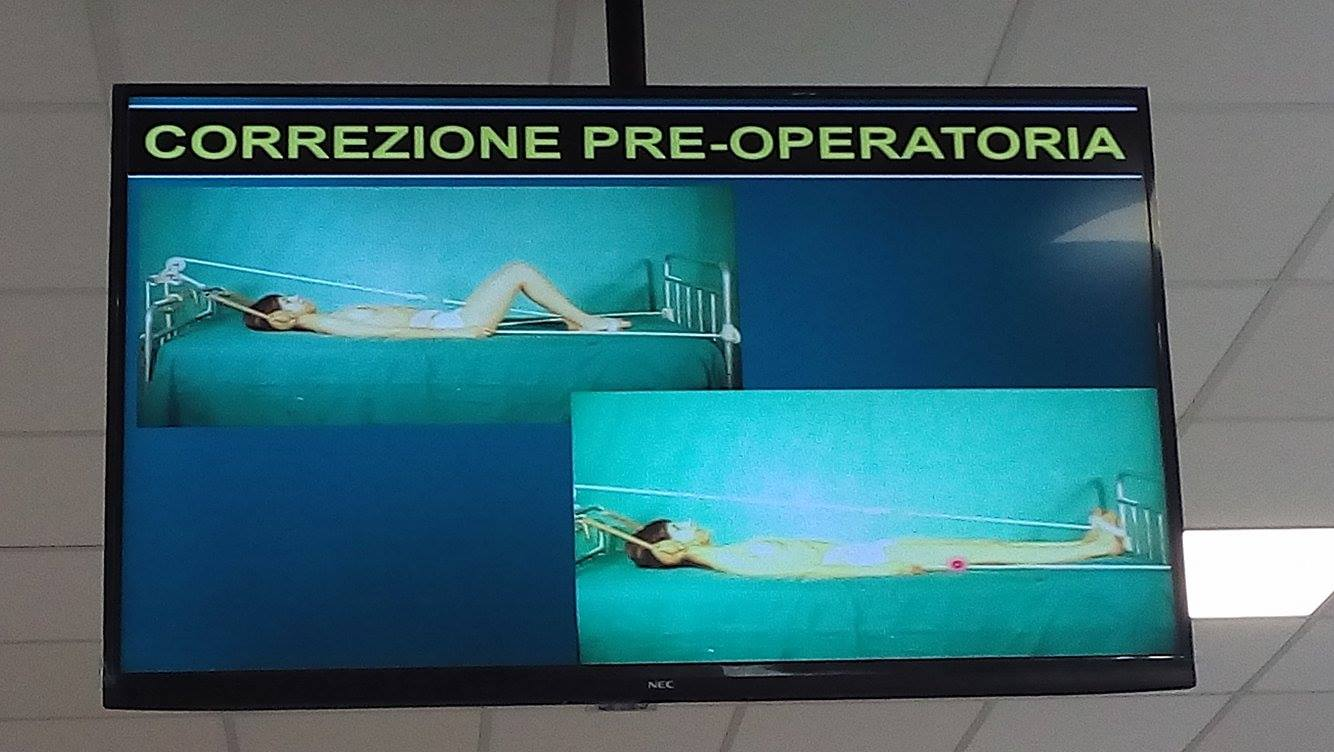
\includegraphics[width=0.4\textwidth]{013/image10.jpeg}
\end{figure}

Un tempo prima del trattamento chirurgico veniva usato questo sistema di corde con una pedana. Era realizzato in maniera tale che il paziente, allungando le gambe, attraverso questa carrucola potesse esercitare una trazione, ovviamente non dolorosa. Serviva per fare in modo che la colonna fosse più elastica così che poi nel campo chirurgico potesse essere corretta meglio. Ricordate che dentro la colonna c'è il midollo spinale e non è una bella idea pensare di ``raddrizzare'' una colonna storta tutta in uno stesso momento perché \emph{una delle complicanze di questo intervento è la paraplegia}. Questo sistema serviva quindi a rendere più elastica la colonna, ma è stato poi abbandonato.

\begin{figure}[!ht]
\centering
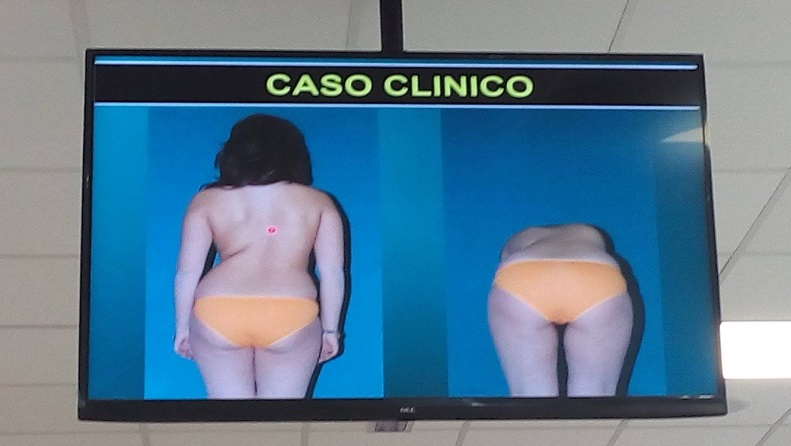
\includegraphics[width=0.4\textwidth]{013/image11.jpeg}
\end{figure}

Esempio classico di scoliosi di una ragazza di 15-16 anni trattata con la chirurgia.

Si tratta di un intervento di \textbf{artrodesi} cche realizza un \textbf{blocco dell'allungamento della colonna}. Questa è la ragione per cui vanno eseguiti quando l'accrescimento è terminato altrimenti il risultato finale potrebbe essere compromesso ad esempio il paziente potrebbe avere le gambe troppo lunghe rispetto al busto Questa è la
radiografia: si vede che è una scoliosi severa in cui anche il polmone è compromesso.

\begin{figure}[!ht]
\centering
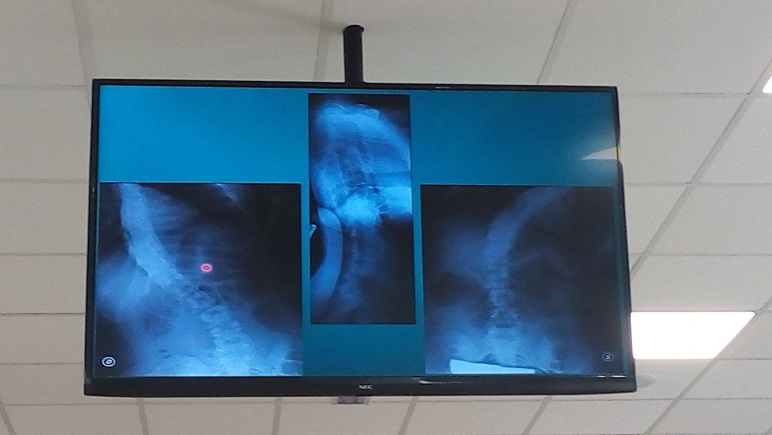
\includegraphics[width=0.4\textwidth]{013/image12.jpeg}
\end{figure}

Ci sono poi i così detti bending test (dall'inglese flettere) o test di elongazione che vengono eseguiti per scegliere l'area in cui agire: \emph{servono per capire quali sono le curve principali}.

\begin{figure}[!ht]
\centering
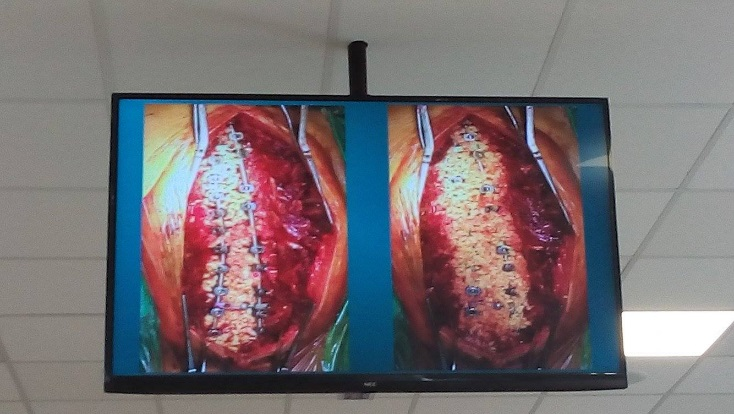
\includegraphics[width=0.4\textwidth]{013/image13.jpeg}
\end{figure}

\begin{figure}[!ht]
\centering
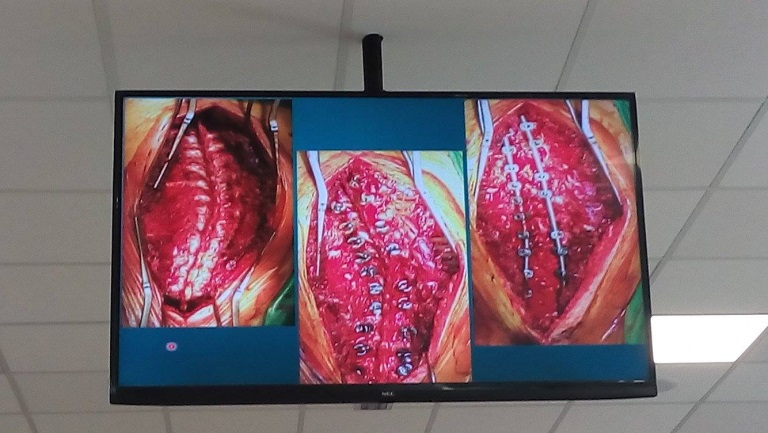
\includegraphics[width=0.4\textwidth]{013/image14.jpeg}
\end{figure}

Bisogna stare attenti a non sbagliare con le scoliosi perché se una forma che necessitava di correzione con trattamento ortopedico, non venisse riconosciuta, poi andrà incontro a peggioramento e quando non si potrà più fare nulla, andrà operata con questo intervento che prevede circa 80cm/un metro di incisione.

Si tratta di un intervento di \textbf{artrodesi posteriore} ovvero \textbf{\emph{blocco dell'area del rachide scelta che comprende ovviamente le curve principali. }}

Solo per realizzare il campo chirurgico sono necessarie due ore: occorre puntellare la colonna con viti e chiodi peduncolari \emph{che penetrano posteriormente attraverso i peduncoli raggiungendo il corpo vertebrale}.
Si costruisce quindi una struttura metallica che \emph{traziona il rachide ed esercita una serie di pressioni e decompressioni localizzate così da correggere le deformità.}

Queste \emph{viti} hanno delle teste con delle scanalature che permettono di raccordarle ( collegarle ) meccanicamente con un sistema di \emph{barre} che possono essere in acciaio o in titanio. Questo è lo strumentario che aiuta nell'artrodesi.

L'artrodesi in sé si effettua \emph{cruentando} l'osso cioè
\emph{scavando la parte posteriore delle vertebre} e si realizza quindi una colata di callo osseo sull'area interessa sfruttando anche del tessuto osseo spongioso prelevato dalla banca dell'osso (la componente inorganica di questo materiale osseo funziona infatti da \emph{osteoinduttore} = stimola la formazione di osso e \emph{osteoconduttore} = intelaiatura per la colonizzazione di cellule del ricevente).

Nell'esempio illustrato dal prof l'osso dei processi spinosi viene rimosso ed usato come materiale per il trapianto d'osso. In questo caso sono state usate nel trapianto d'osso anche delle teste di femore prelevate da pazienti operati di coxartrosi con protesi d'anca.
Quest'osso viene spezzettato: si decorticano le lamine e viene realizzata la colata di callo osseo sia con l'osso delle spinose sia in parte con l'osso spezzettato del femore (provenienti da banche dell'osso).

\emph{Quello che tiene meccanicamente nel tempo non è l'acciaio o il titanio, ma è l'artrodesi che finisce per inglobare la struttura fatta di viti e barre}: paradossalmente questa strumentazione, nel momento in
cui si è creata una distesa di osso, potrebbe anche essere tolta. Non si fa ovviamente perché l'osso ingloba tutto il metallo e sarebbe un intervento più impegnativo di quello iniziale.

La mobilità è solo lievemente ridotta, ma la qualità della vita è nettamente migliorata rispetto a prima anche in vista delle complicanze artrosiche della scoliosi.

Ci potrebbero essere delle complicanze perché se non tiene
l'impalcatura, l'osso si potrebbe rompere mentre a volte si ha una pseudoartrosi: se l'osso non si fonde, lo strumentario per conto suo non riesce a resistere a tutte le sollecitazioni di una vita normale e prima o poi si rompe, con perdita della correzione.

\begin{figure}[!ht]
\centering
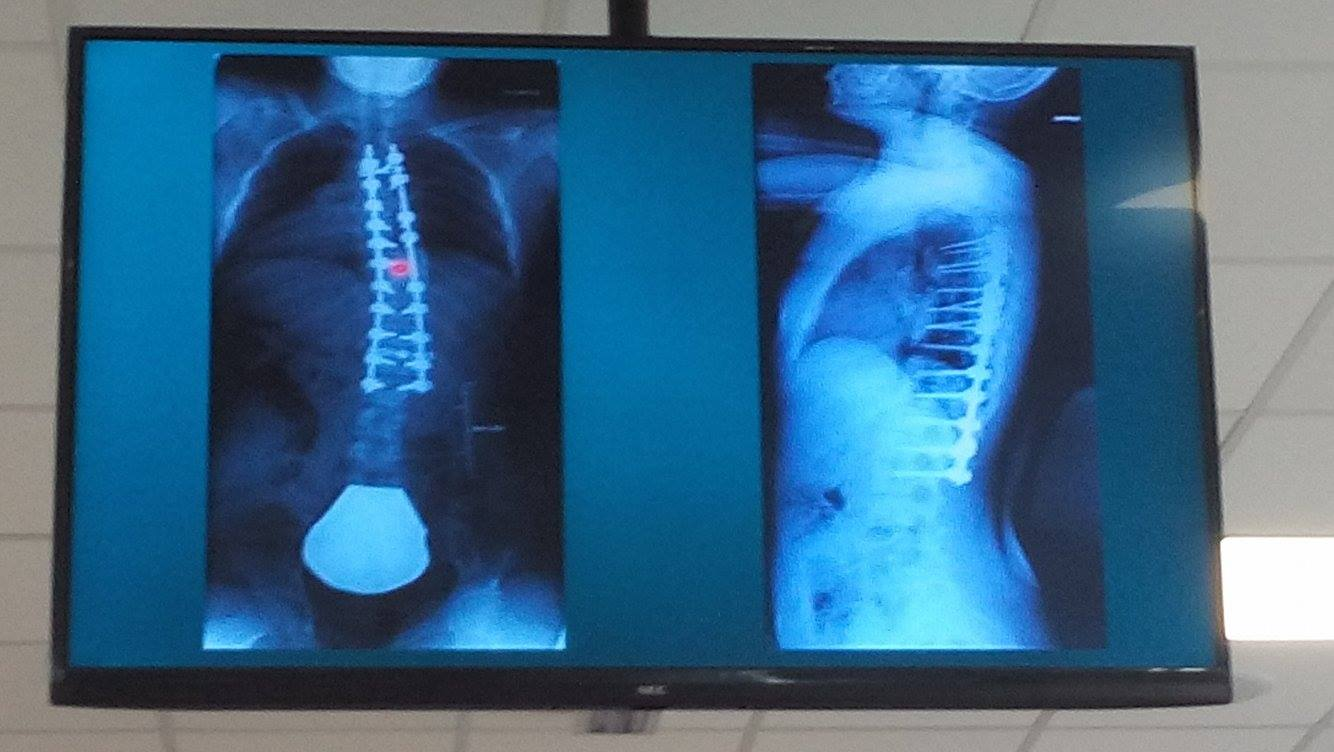
\includegraphics[width=0.4\textwidth]{013/image15.jpeg}
\end{figure}

Qui vediamo il risultato finale: le viti partono da dietro e terminano nel corpo vertebrale. Bisogna stare attenti a non piantare queste viti nel midollo spinale. Quest'area di artrodesi \textbf{\emph{viene bloccata}}, ma è ovvio che questa parte di colonna dal momento che non è così mobile non darà grossi danni ai fini ad esempio del raccogliere una matita. Bloccando però fino alla zona lombare, le ultime quattro vertebre libere sicuramente non godono e vanno incontro a un processo di degenerazione.

Sono interventi che devono essere fatti in centri specializzati. I primi interventi si facevano con dei chiodi che prevedevano sei mesi di gesso: due mesi stando a letto, due mesi iniziando a muoversi e due mesi
svolgendo le normali attività. Oggi invece con i nuovi strumentari, siccome viene distribuito tutto a vari livelli, i pazienti possono rimettersi in piedi dopo 4-5 giorni a seconda di quanto sangue abbiano perso.

Qualche volta le cicatrici non sono molto evidenti: quando dopo l'intervento erano previsti sei mesi di gesso, le cicatrici erano migliori perché erano protette da questo. Con i nuovi interventi, a seguito dei quali il paziente può muoversi subito, i lembi della ferita si muovono di più e la cicatrice tende a dare reazioni cheloidee più significative.

\begin{figure}[!ht]
\centering
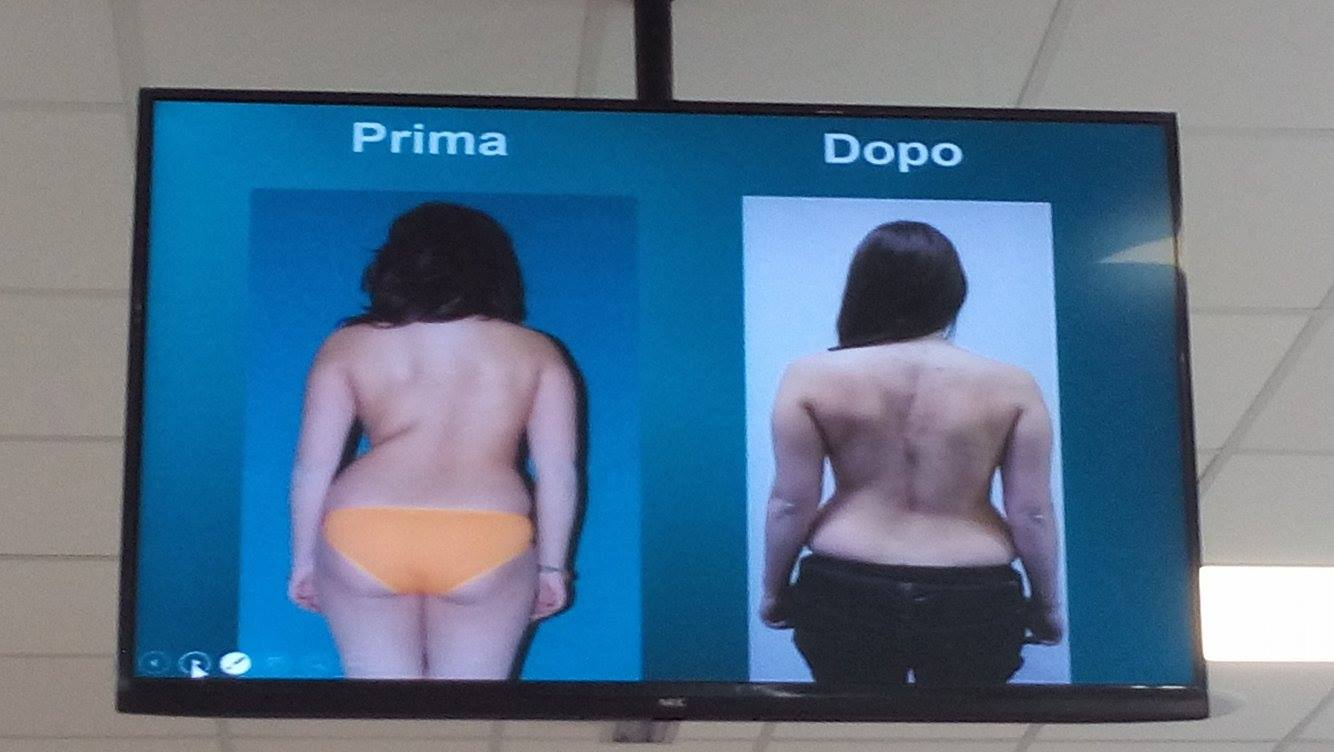
\includegraphics[width=0.4\textwidth]{013/image16.jpeg}
\end{figure}

Qui vediamo il prima e dopo: osserviamo come la colonna si è de-ruotata.
Questo non è un discorso estetico, ma soprattutto funzionale. La gabbia toracica si è normalizzata e il polmone risente meno della costrizione.
In ortopedia l'estetica conta poco. L'ortopedico è un chirurgo funzionale.

Il messaggio fondamentale è che la scoliosi è una cosa grave e anche se il 99\% degli ortopedici ha a che fare con le forme che non peggiorano, bisogna sapere che esistono anche forme che peggiorano e che vanno trattate nel modo adeguato.

Domanda: ma le viti messe durante l'intervento sono riassorbibili? No, anche se meccanicamente si potrebbero anche rimuovere (è capitato qualche volta perché possono dare fastidi e gonfiori). Quello che tiene infatti è l'artrodesi! Liberare ogni vite dall'osso sarebbe un
intervento lungo e pericoloso che non viene fatto, se non per necessità.

Domanda: ci possono essere complicanze a livello di midollo osseo? Sì, se stiri troppo lo mandi in paresi. Ci sono due modi per capire se c'è stata o meno una lesione spinale:

\begin{itemize}
\item
  Quando non esistevano i potenziali evocati, si svegliava il malato attraverso un alleggerimento dell'anestesia e un'infermiera con un cocker (pinza con i denti) andava a dare morsi sugli alluci. Se il malato muoveva le gambe, voleva dire che magari potevi andare a tirare ancora un po'
\item
  Oggi si va in sala operatoria con dei neurologi e si sfruttano i \textbf{potenziali evocati}: senza svegliare il malato si usano gli elettrodi e un'apparecchiatura di elettrofisiologia così si riesce a capire quanto si può stirare il midollo.
\end{itemize}

Al prof è capitato una solo volta di dover tornare in sala tre ore dopo l'intervento per un problema di coagulazione intravasale disseminata. Ha dovuto riaprire e detendere, ma non per un problema di trazione bensì di coagulazione. Erano i primi tentativi che si facevano per il recupero
intraoperatorio del sangue: succedeva che per rendere il sangue più fluido, venivano aggiunti degli anticoagulanti al sangue che veniva riciclato e reinfuso. Purtroppo questi scatenarono una coagulazione intravasale disseminata con consumo di tutti i fattori della coagulazione e sanguinamento eccessivo. Si creò così un ematoma nel
canale vertebrale.
\\\\
\emph{Domanda: esiste un cut-off di angolo di scoliosi a partire dal quale è consigliato il trattamento ortopedico? No, perché il valore assoluto non è significativo. Dipende tutto dall'età anagrafica e soprattutto dall'età di accrescimento scheletrico. E' chiaro però che, se il tessuto familiare del bambino con una scoliosi di 20 gradi non garantisce una corretta terapia ortopedica, conviene operare subito per non perdere tempo prezioso.}


\section{Torcicollo}

\emph{Il prof ci tiene a sottolineare che per lui, in sede di esame, è importantissimo sapere la definizione: così facendo ci si è quasi assicurati la promozione.}

Il torcicollo viene definito come una deviazione laterale permanente (quindi deformità) del capo e del collo.

\emph{Si tratta quindi di una deformità dove per deformità si intende una posizione o situazione che l'individuo non può correggere volontariamente (a differenza di una postura, o di un atteggiamento).
Nel caso del torcicollo, infatti, si parla di una patologia vera e propria.}

La classificazione lo distingue in:

\begin{itemize}
\item
  \textbf{Congenito}, che può essere:
\begin{itemize}
\item
  Miogeno che (lo sottolineiamo fin da subito) non dà un gran problema funzionale, ma soprattutto di tipo estetico
\item
  Osseo
\end{itemize}
\item
  \textbf{Acquisito}, che può essere:
\begin{itemize}
\item reumatico
\item osteoarticolare
\item nervoso
\item isterico
\item oculare
\item otogeno
\item miopatico.
\end{itemize}
\end{itemize}

Questi hanno valenza per una diagnosi differenziale: in tutte queste possiamo avere caratteristiche simile al torcicollo inteso come deformità sia ossea che miogena.

\emph{La classificazione è utile dal punto di vista clinico perché aiuta nella diagnosi differenziale. Infatti spesso in ortopedia si presentano casi che hanno in comune sintomi (tutti i torcicolli si presentano come deviazioni del collo, le scoliosi come deviazioni della colonna vertebrale, ecc.), ma che hanno eziologie ed origini diverse: ci possono essere patologie secondarie, primitive o anche idiopatiche. Sulla base delle informazioni derivanti dalla causa della patologia possiamo mettere a punto un trattamento adeguato.}

\subsection{Torcillo osseo}

Deriva da \textbf{\emph{malformazioni congenite vertebrali}} sovrapponibili a quelle delle scoliosi.

\begin{figure}[!ht]
\centering
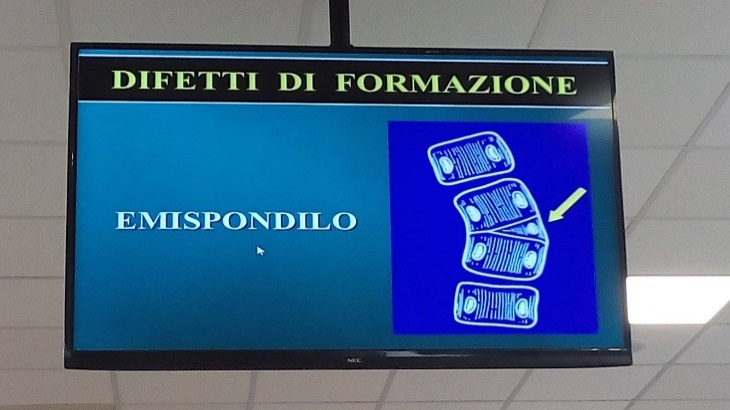
\includegraphics[width=0.4\textwidth]{013/image17.jpeg}
\end{figure}

\begin{figure}[!ht]
\centering
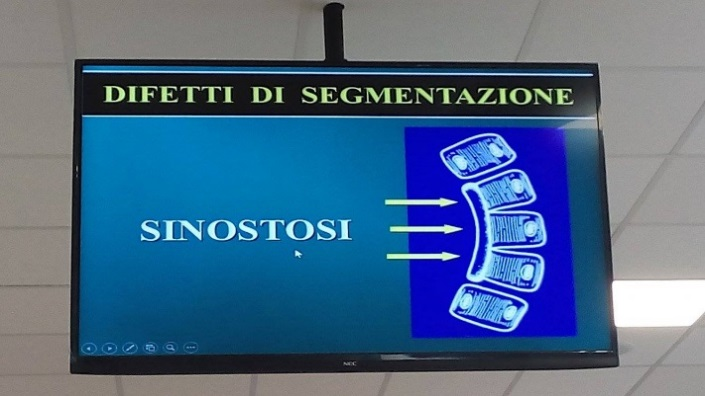
\includegraphics[width=0.4\textwidth]{013/image18.jpeg}
\end{figure}

Può derivare da:

\begin{itemize}
\item
  \textbf{Difetti di formazione}: si forma solo una mezza vertebra e non l'intera ovvero una struttura detta emispondilo
\item
  \textbf{Difetti di segmentazione} quindi sinostosi ovvero fusioni che \emph{in realtà sono mancate separazioni tra un osso e l'altro perciò difetti di segmentazione: le vertebre sono formate, ma non separate e possono essere fuse in corrispondenza o dell'intera superficie di confine o di una parte di questa. }
\end{itemize}

\begin{figure}[!ht]
\centering
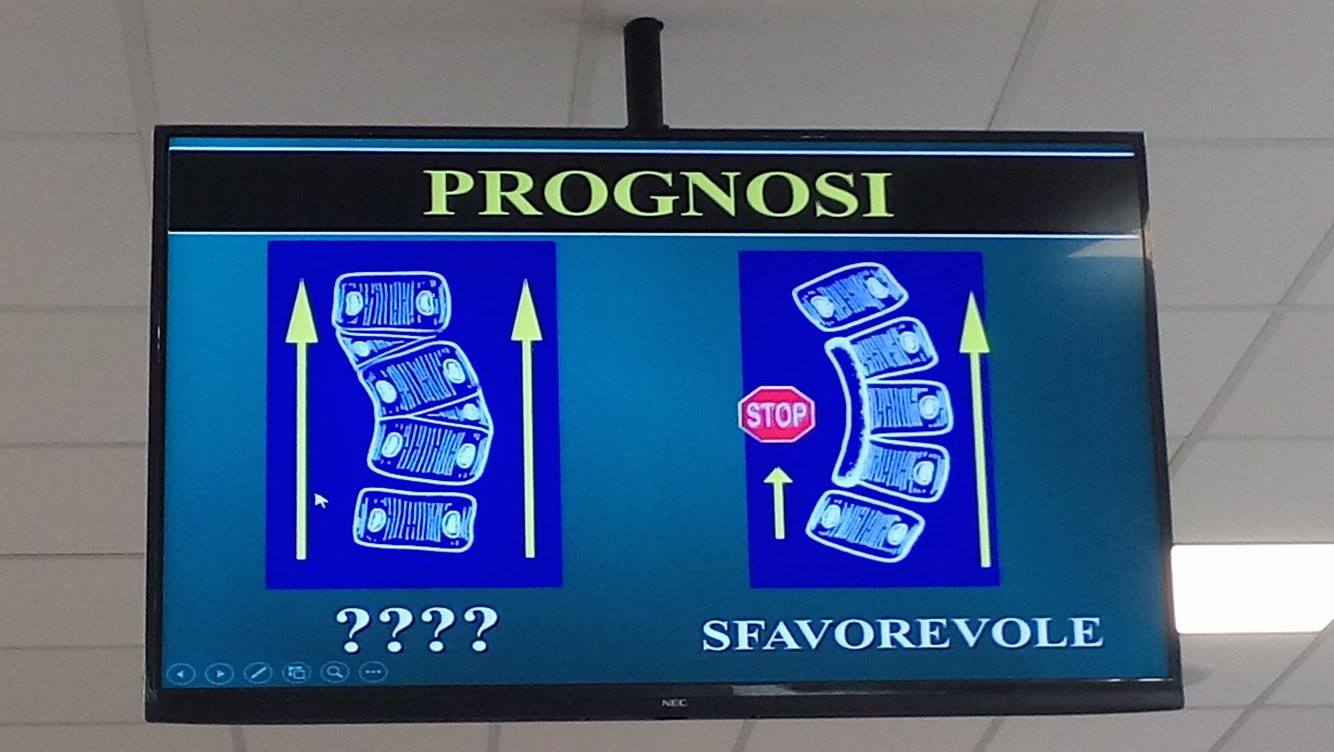
\includegraphics[width=0.4\textwidth]{013/image19.jpeg}
\end{figure}

La distinzione fra emispondilo e sinostosi è importante per la prognosi:

\begin{itemize}
\item
  Per l'emispondilo \emph{può esserci la possibilità che l'individuo non cresca con una deviazione del collo} perché per esempio possono esserci due emispondili in grado di controbilanciarsi e riassettare la linea del collo. In sostanza si ha una \emph{compensazione} del difetto.
\item
  Per la sinostosi la prognosi è sicuramente \emph{più sfavorevole} perché \emph{l'arresto della crescita della porzione delle vertebre che non si è segmentata è parallelo alla progressione della crescita della porzione segmentata.} La tendenza alla flessione laterale del capo e del collo peggiorerà
\end{itemize}

All'esame clinico vediamo:

\begin{itemize}
\item
  Una \textbf{\emph{mobilità limitata del collo}} che però si vede meno nel miogeno
\item
  \textbf{\emph{Assenza dei segni di retrazione dello sternocleidomastoideo}} che invece caratterizzano il torcicollo miogeno.
\end{itemize}

\begin{figure}[!ht]
\centering
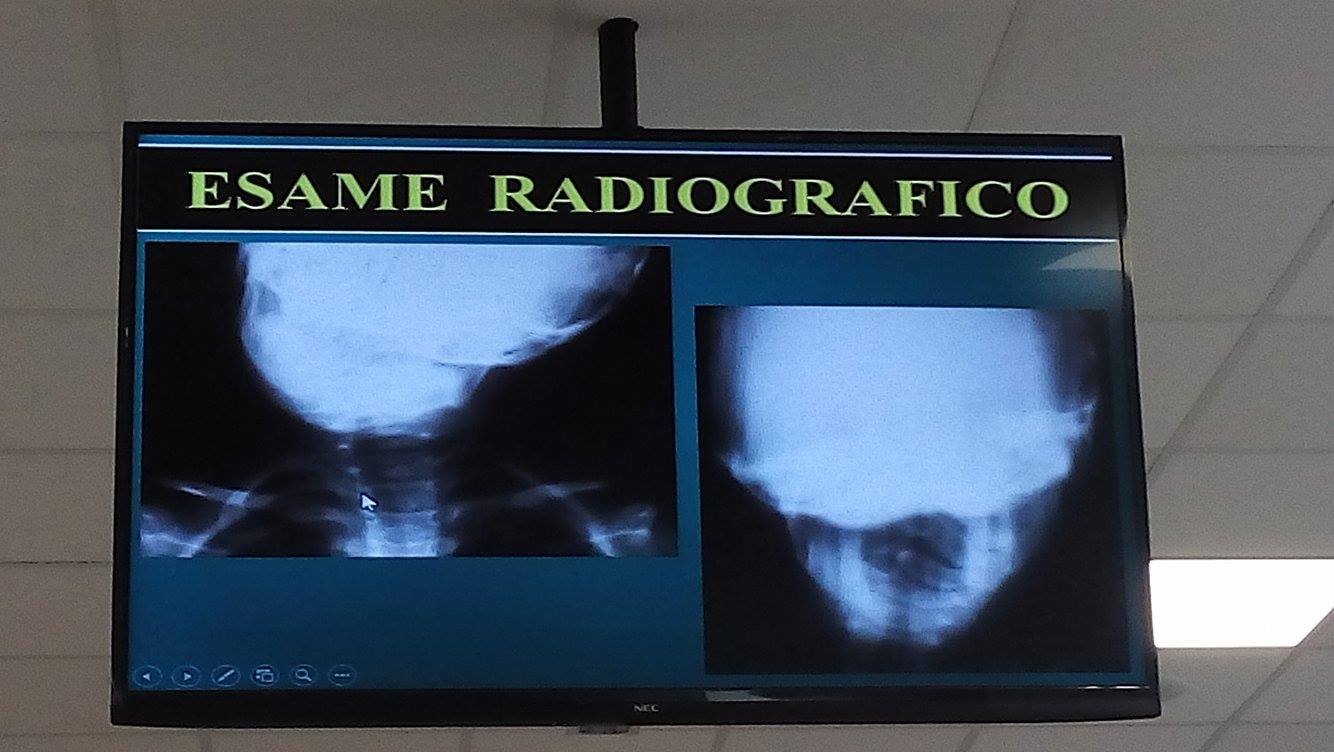
\includegraphics[width=0.4\textwidth]{013/image20.jpeg}
\end{figure}

Vediamo un esempio di radiografia. Studiare il rachide dal punto di vista radiografico è praticamente impossibile! Se si volesse approfondire lo studio, bisognerebbe eseguire una TAC.

Ci si accorge del problema osseo perché quando muoviamo la testa del bambino, l'arresto è più brusco, il movimento è più limitato. Mentre nel \textbf{miogeno} vedremo che il \textbf{collo è più elastico} perché la colonna è normale.

\subsection{Torcicollo miogeno}

Deriva da una \textbf{\emph{retrazione del muscolo sternocleidomastoideo}} ed è detto anche ostetrico o congenito-muscolare (congenito significa connatale e non ereditario).

Può essere dovuto ad alterazioni prevalenti del:

\begin{itemize}
\item
  Capo clavicolare
\item
  Capo sternale
\item
  Capo mastoideo
\item
  Di tutti e tre (il muscolo ha tre inserzioni: sternale, clavicolare e mastoidea).
\end{itemize}

\begin{figure}[!ht]
\centering
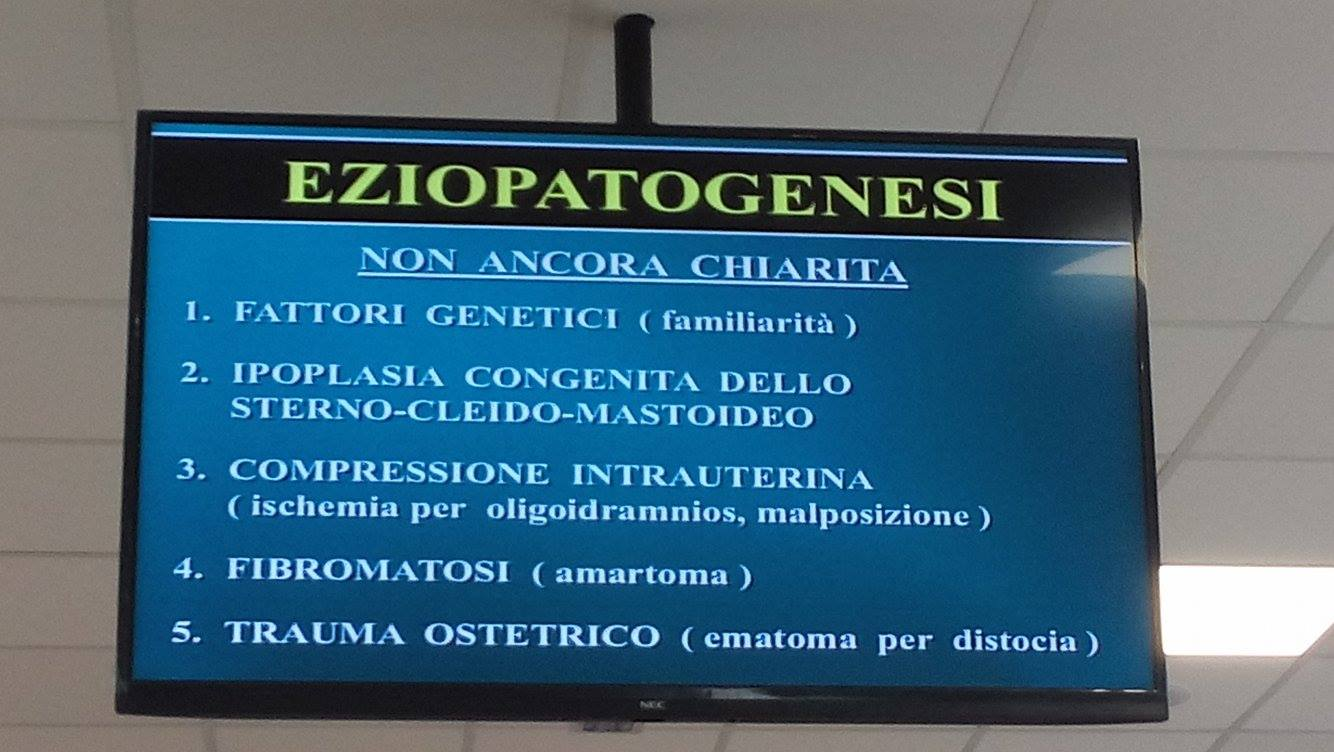
\includegraphics[width=0.4\textwidth]{013/image21.jpeg}
\end{figure}

L'eziopatogenesi non è chiara:

\begin{itemize}
\item
  Fattori genetici (\emph{di familiarità, non ereditarietà}) non ancora scoperti
\item
  Ipoplasia congenita del muscolo sternocleidomastoideo (\emph{anche se questa condizione da sola non spiega la progressiva retrazione del muscolo che invece si presenta nel torcicollo})
\item
  Compressione intrauterina: \emph{per \emph{ischemia da oligoidramnios} ovvero quantità esigua di liquido amniotico che condiziona determinate posizioni anomale del feto che riducono l'apporto ematico alla massa muscolare oppure \emph{per mal posizione}}
\item
  Fibromatosi che a oggi rappresenta la teoria più accreditata (\emph{per amartoma si intende un lesione pseudo tumorale, non maligna, dovuta allo sviluppo delle cellule normali di quel tessuto in maniera anarchica, ma non si tratta di cellule anaplastiche. Sia l'amartoma che l'ematoma tendono a rapprendersi nel tempo e quindi a retrarre il muscolo})
\item
  Trauma ostetrico per questo detto anche ostetrico. Era dovuto ad un ematoma da distocia: in parti detti distocici veniva usato uno strumento chiamato forcipe che afferrava il feto per la testa. Si creavano o \emph{trazioni eccessive sul collo} o \emph{una compressione sul muscolo sternocleidomastoideo}. Questo creava un ematoma che con l'andare del tempo si organizza, diventava fibroso e si rapprendeva così da accorciare il muscolo.
\end{itemize}

\begin{figure}[!ht]
\centering
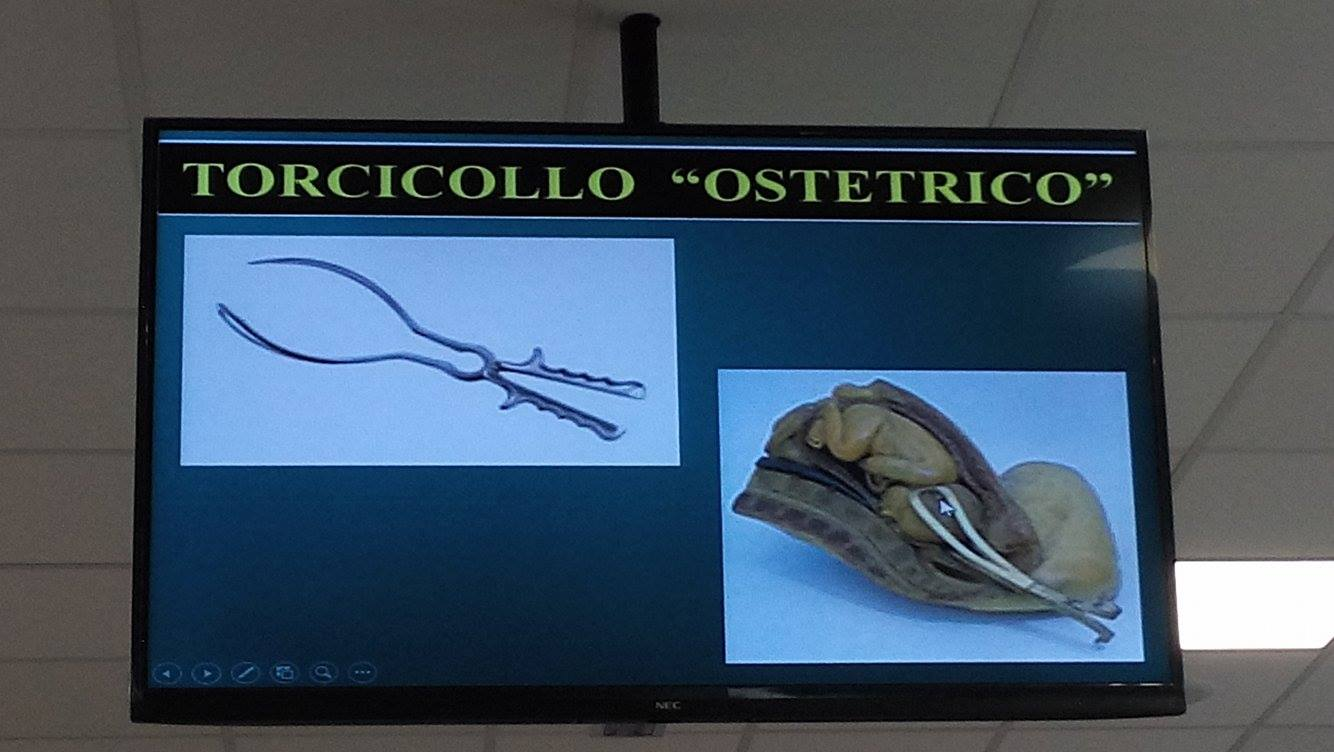
\includegraphics[width=0.4\textwidth]{013/image22.jpeg}
\end{figure}

\emph{Anche in caso di parto non distocico si poteva avere torcicollo: si è notato che questo ematoma si può formare anche in neonati con parto normale o cesareo quindi il traumatismo può non essere la causa.}

L'ipotesi più accreditata è quello di un \emph{amartoma} cioè un'isola di tessuto indifferenziato che con il tempo da un punto di vista biologico, ma soprattutto meccanico, ha la stessa evoluzione dell'ematoma cioè si rapprende e dà una retrazione del muscolo sternocleidomastoideo.

\subsubsection{Quadro clinico ed evoluzione}

\begin{figure}[!ht]
\centering
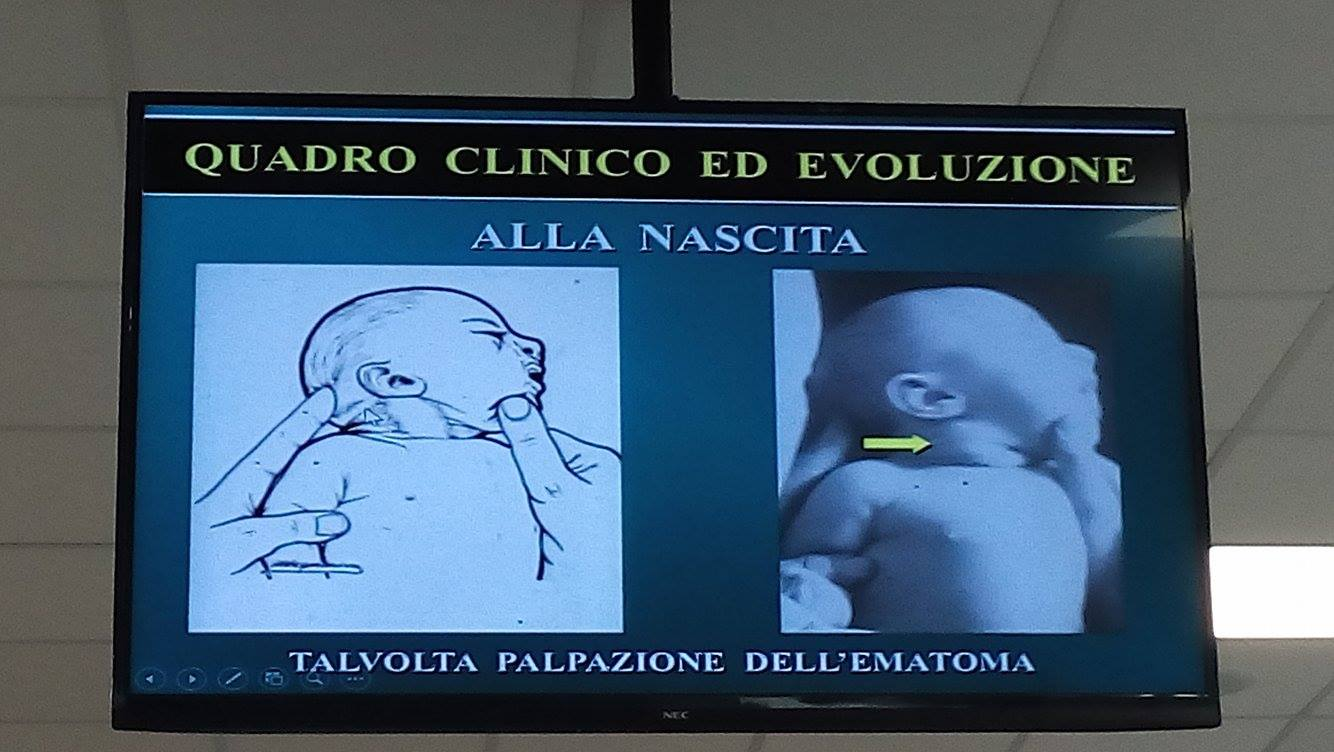
\includegraphics[width=0.4\textwidth]{013/image23.jpeg}
\end{figure}

\emph{Il quadro clinico del torcicollo miogeno è povero di segni alla nascita:} non si vede un granché. \emph{A volte è palpabile l'ematoma o l'amartoma al collo}, si può percepire un pallino, ma di fatto non ce ne accorgiamo. La diagnosi è clinica mentre gli esami strumentali sono difficili da compiere alla nascita: al massimo un'ecografia ci può far vedere o l'amartoma o l'ematoma.

\begin{figure}[!ht]
\centering
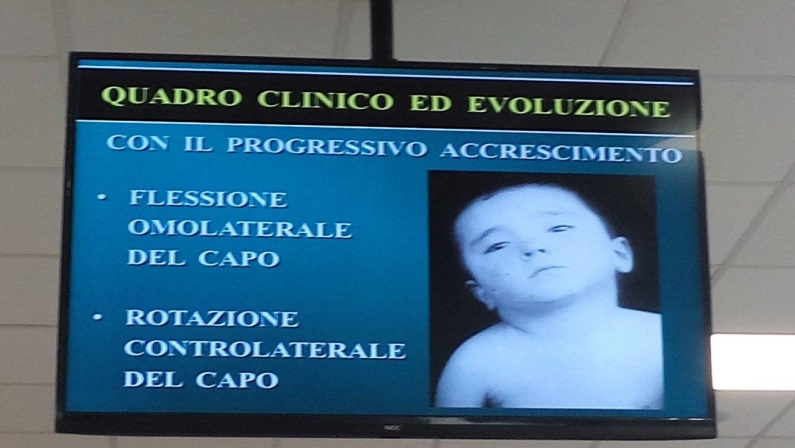
\includegraphics[width=0.4\textwidth]{013/image24.jpeg}
\end{figure}

Dopo con l'accrescimento, vediamo che dalla parte dove ``tira'', il volto e il collo si sviluppano meno. Dall'altra parte invece crescono di più. Si inizia a vedere l'atteggiamento della testa in flessione dalla parte del muscolo interessato e di rotazione dalla parte opposta.
Infatti col progressivo accrescimento si verifica:

\begin{itemize}
\item
  \emph{Flessione omolaterale} del capo
\item
  \emph{Rotazione controlaterale} del capo
\end{itemize}

\begin{figure}[!ht]
\centering
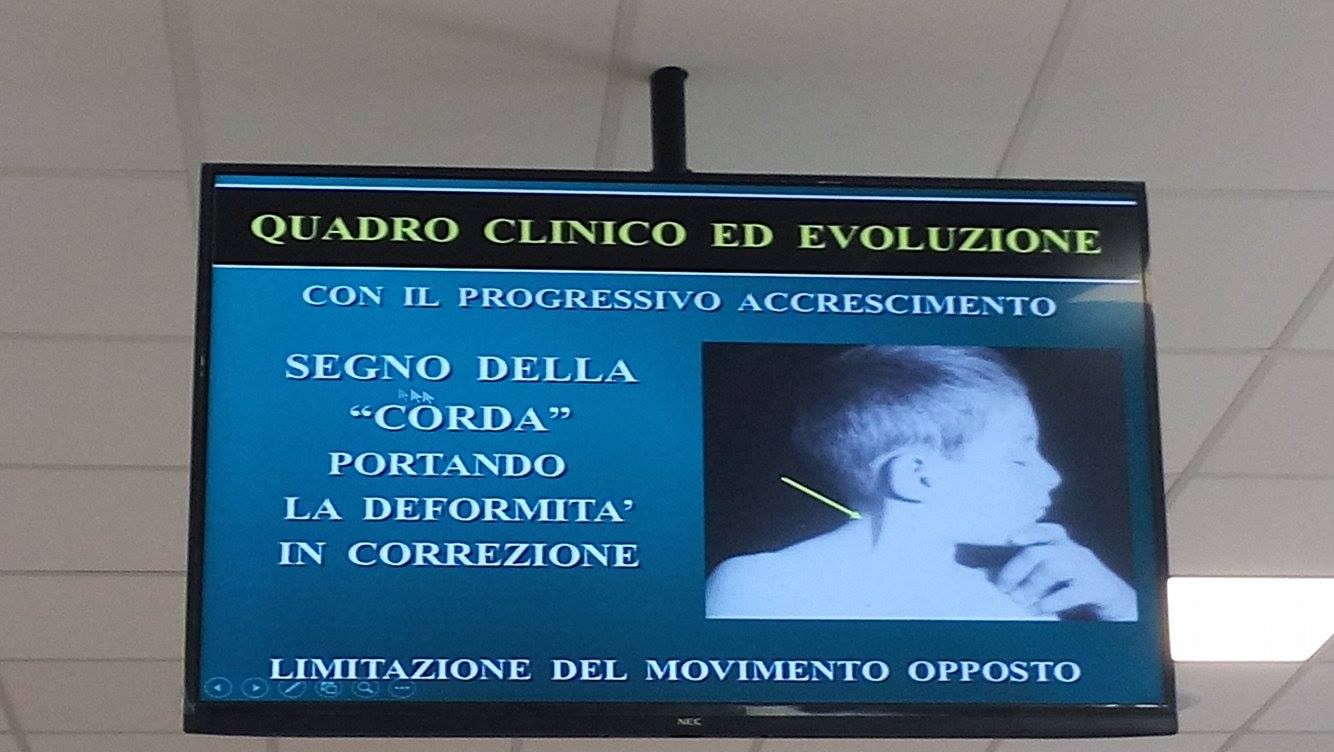
\includegraphics[width=0.4\textwidth]{013/image25.jpeg}
\end{figure}

Queste condizioni tendono a peggiorare con l'accrescimento e poi compare il \textbf{segno della corda} (attorno ai 5-6-7 anni di età): tenendogli ferme le spalle, la testa è fatta ruotare dalla parte opposta al muscolo affetto portando così la deformità in correzione. \emph{Forzando la rotazione dalla parte della deformità, ho la limitazione del movimento opposto, e si può rilevare tensione in superficie in corrispondenza del muscolo retratto (lo sternocleidomastoideo)}. C'è una limitazione del movimento opposto, ma è una limitazione che, rispetto al torcicollo
osseo, è molto più elastica. \emph{La limitazione nel caso del torcicollo miogeno è di tipo elastico, differente dal caso del torcicollo osseo nel quale non ci sarebbe segno della corda e inoltre la limitazione di movimento sarebbe molto più dura.}

\begin{figure}[!ht]
\centering
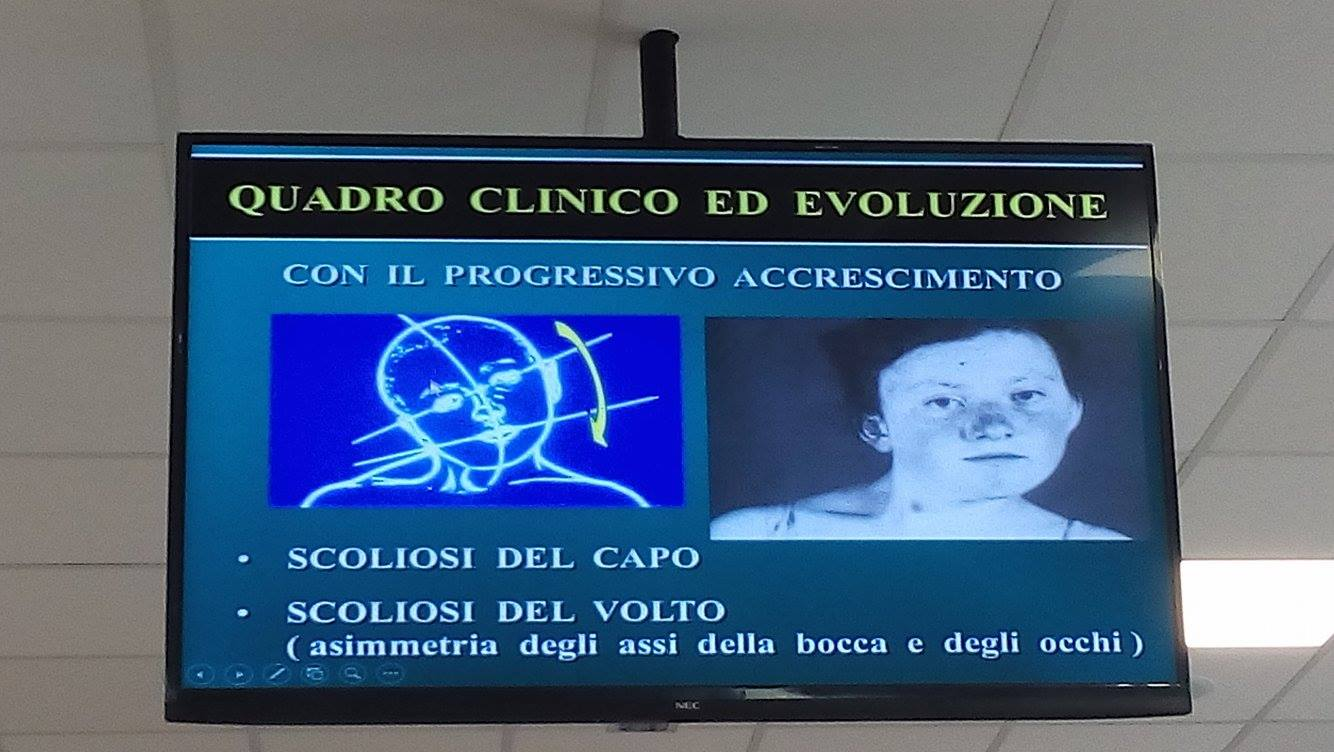
\includegraphics[width=0.4\textwidth]{013/image26.jpeg}
\end{figure}

Con il passare del tempo si assiste ad un'alterazione delle linee di accrescimento osseo \emph{che si strutturano secondo linee di forza alterate}: dalla parte del muscolo interessato c'è un freno ai vettori dell'accrescimento mentre dalla parte opposta no. Come conseguenza di questa crescita asimmetrica (il capo cresce più dalla parte opposta) avremo una scoliosi del capo detta \emph{plagiocefalia} e una scoliosi del volto detta \emph{plagioprosopia} ovvero asimmetria degli assi della bocca e degli occhi che si vede tirando due linee immaginarie: una che passa gli occhi e una per gli angoli della bocca. Queste linee non sono parallele, ma sono convergenti dalla parte del muscolo interessato.

\begin{figure}[!ht]
\centering
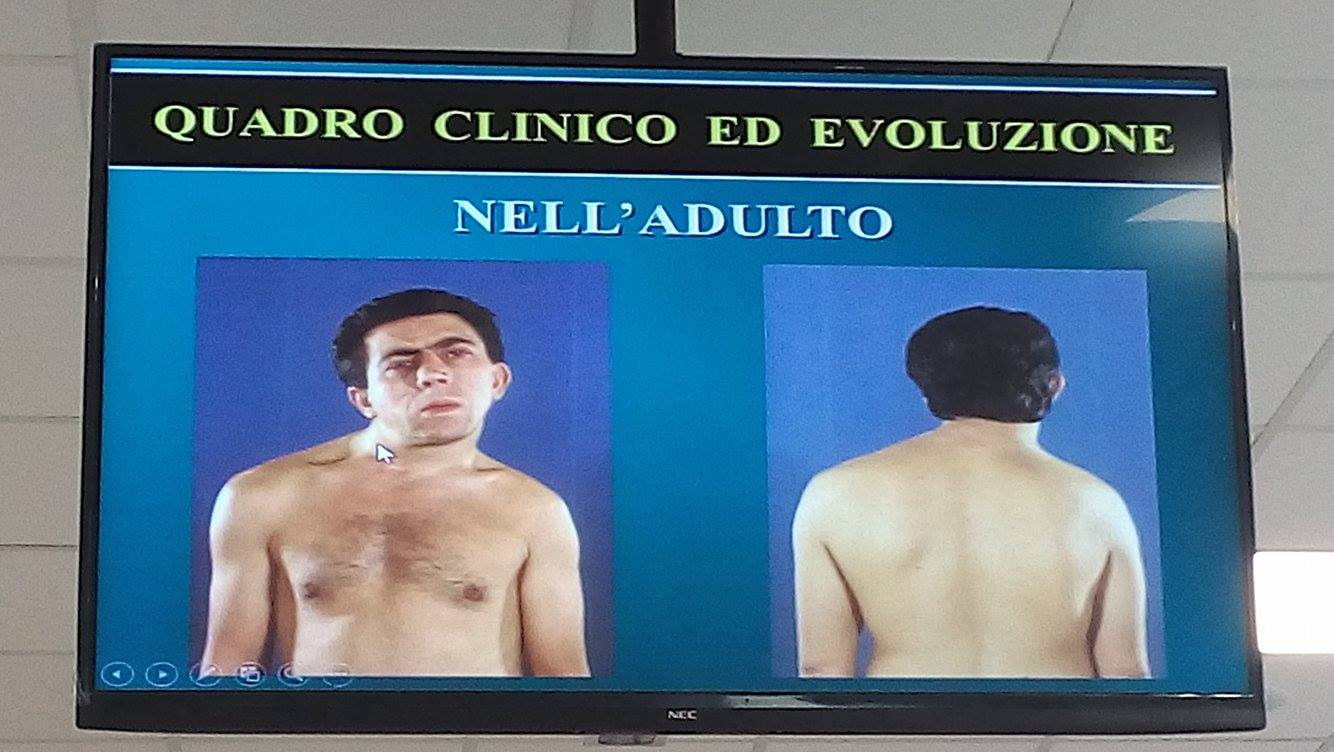
\includegraphics[width=0.4\textwidth]{013/image27.jpeg}
\end{figure}

Vediamo un esempio di come si presenta nell'adulto. È molto difficile vederli dopo l'infanzia. Qui si vede molto bene il segmento che tira. A questo punto non si fa più nulla perché al di là del problema estetico e della limitazione della rotazione del collo, non ci sono problematiche
importanti.

\subsubsection{Trattamento}

Il trattamento non è solitamente necessario ed è solo chirurgico. Si esegue la \textbf{tenotomia tripolare}: si tagliano tutti e tre i poli del tendine del muscolo (sostanzialmente significa allungarlo, ma non potendolo allungare, si taglia). Si taglia a livello di inserzione
mastoide, sternale e scapolare.

\begin{figure}[!ht]
\centering
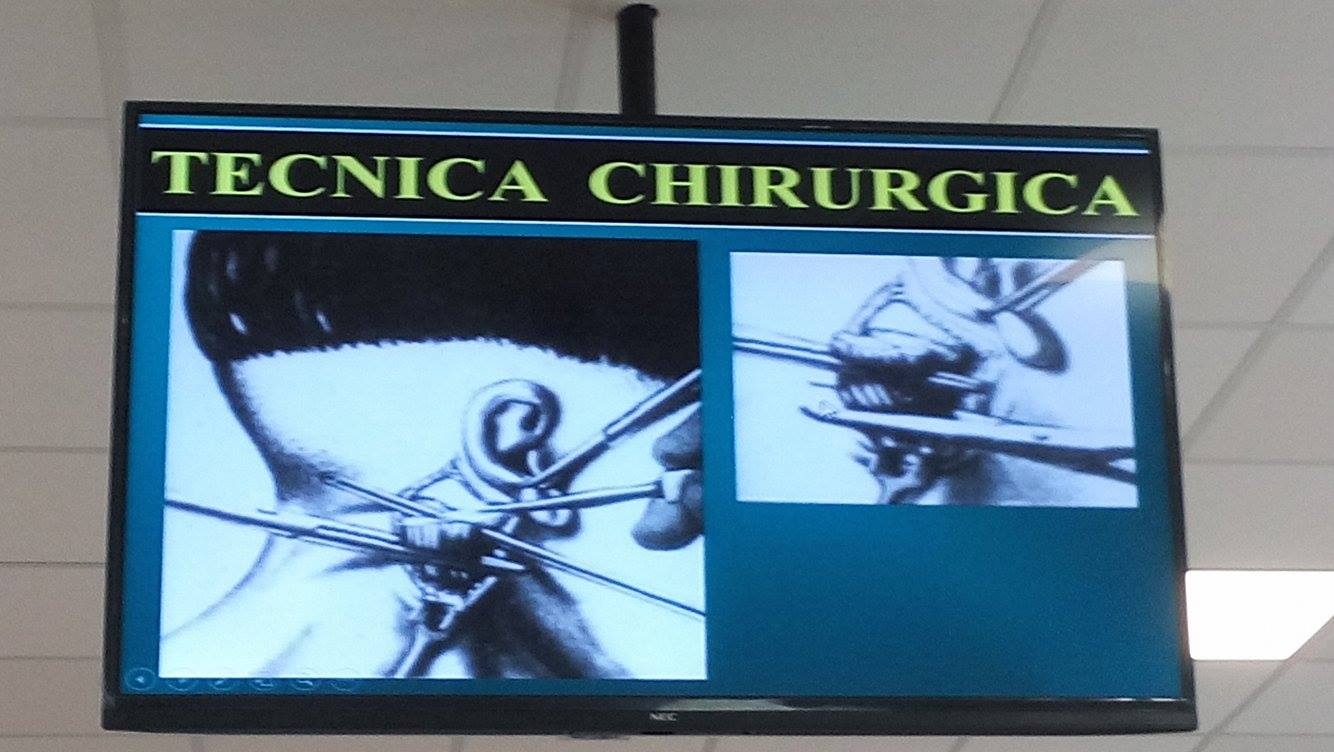
\includegraphics[width=0.4\textwidth]{013/image28.jpeg}
\end{figure}

Vediamo che l'orecchio viene divaricato, con uno specillo si prende il tendine che viene prima isolato con un cocker e poi tagliato così da eliminare un pezzo di muscolo. La stessa cosa viene fatta poi a livello clavicolare e sternale.

Non è un intervento semplice: bisogna rimanere superficiali dal momento che sotto ci sono strutture come la succlavia che non vanno tagliate.

\begin{figure}[!ht]
\centering
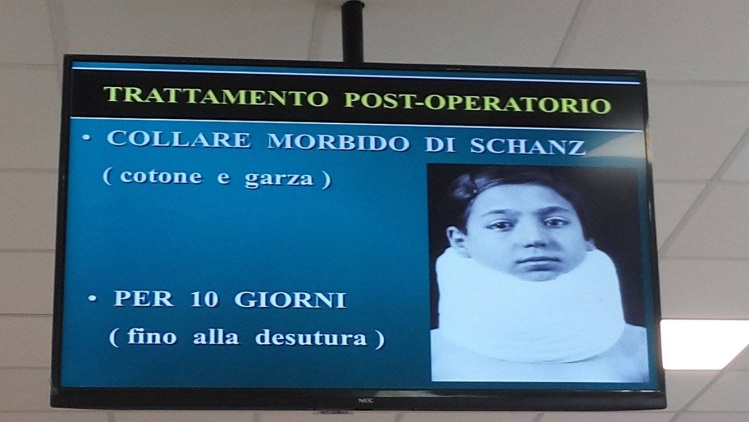
\includegraphics[width=0.4\textwidth]{013/image29.jpeg}
\end{figure}

In seguito alla tenotomia, per evitare la recidiva, vi è anche l'asportazione di 1 cm di tendine da tutti e tre i poli perché assieme al trattamento post-operatorio, l'asportazione del cm evita che il muscolo si ``riattacchi'' dov'era prima (recidiva).

Nel post-operatorio si utilizza il \emph{collare morbido di Schanz} (che supporta il collo) finché le ferite sono fresche e finché non si fa la desutura (circa dieci giorni). È un collare di ovatta, cotone da gesso e
garza.

\begin{figure}[!ht]
\centering
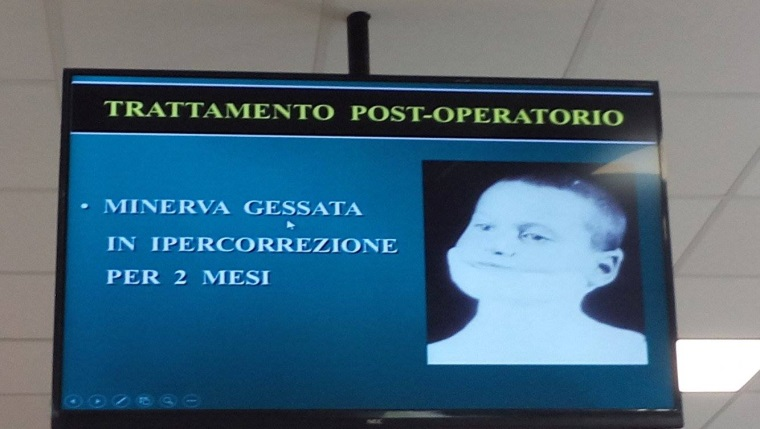
\includegraphics[width=0.4\textwidth]{013/image30.jpeg}
\end{figure}

Importante è l'uso di una \emph{minerva gessata} (apparecchio gessato Minerva) che tiene immobilizzato il capo e il collo in \textbf{ipercorrezione} cioè dal lato opposto alla parte lesa quindi \emph{il collo sarà in flessione controlaterale e rotazione omolaterale} (la deformità è il contrario). Questo dispositivo viene mantenuto per 2 mesi. Sono libere le braccia fino allo sterno e la testa viene immobilizzata.

L'asportazione di 1 cm dai poli, la tenotomia e la posizione per circa due mesi in ipercorrezione faranno sì che i due poli non si riattacchino esattamente dove li abbiamo tagliati.

L'uso della minerva ingessata nel post-operatorio è il motivo per cui l'intervento chirurgico non può essere eseguito prima che il bambino abbia raggiunto una \emph{autonomia alimentare} cioè prima dei due /due
anni e mezzo di età perché prima di allora i bambini si nutrono prevalentemente con la suzione per cui con l'apparecchio gessato risulterebbe difficoltosa la gestione alimentare.

Quindi fino ai due anni cosa faccio?

\begin{itemize}
\item
  Collare di Schanz
\item
  Collare in plastica
\item
  Caute mobilizzazioni del capo
\end{itemize}

Tutto per limitare l'aggravamento della retrazione.

\subsection{Torcicollo acquisito}

\subsubsection{Torcicollo reumatico}

\begin{figure}[!ht]
\centering
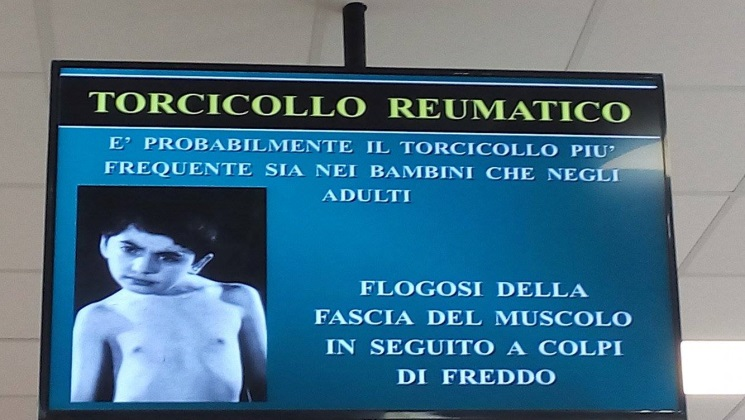
\includegraphics[width=0.4\textwidth]{013/image31.jpeg}
\end{figure}

È il più frequente, si tratta di un'infiammazione del perimisio (ovvero la guaina) del muscolo a seguito di colpi di freddo dati da aria condizionata, finestrino aperto, ecc. Basta prendere un'aspirina.

\subsubsection{Torcicollo osteoarticolare}

Può essere dato da

\begin{itemize}
\item
  \emph{Alterazioni ossee}: rachitismo, lesioni infiammatorie, neoplasie, traumatismi
\item
  \emph{Alterazioni articolari}: spondilite anchilopoietica, artrite reumatoide, ernia discale.
\end{itemize}

\begin{figure}[!ht]
\centering
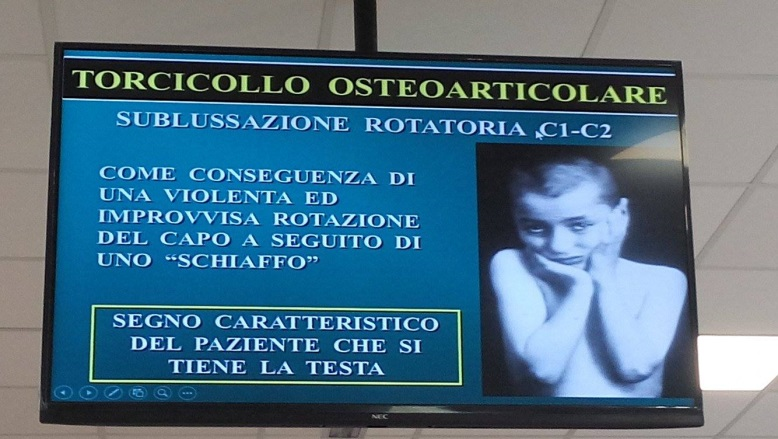
\includegraphics[width=0.4\textwidth]{013/image32.jpeg}
\end{figure}

In questi casi esiste un duplice meccanismo: c'è la lesione organica, ma anche la contrattura antalgica, per cui si crea torcicollo per avere meno dolore.

Una causa relativamente comune può essere la sublussazione rotatoria C1-C2, in questo caso c'è un segno caratteristico: il \textbf{paziente che si tiene la testa}. Non è grave ma va riconosciuto.

Quest'ultimo si osserva spesso nei bambini: a seguito di uno schiaffo, il bambino gira violentemente la testa e si crea una sublussazione rotatoria tra atlante ed epistrofeo. Il bambino si tiene la testa perché il rachide cervicale non riesce a tenerla su. Classica condizione di insufficienza del rachide che va indagata perché potrebbe sottendere una situazione più grave (va messa in relazione con gli eventi).

\subsubsection{Torcicollo nervoso}

Per paralisi, spasticismo, nevralgia del trigemino o altre cause.

\subsubsection{Torcicollo isterico}

\begin{figure}[!ht]
\centering
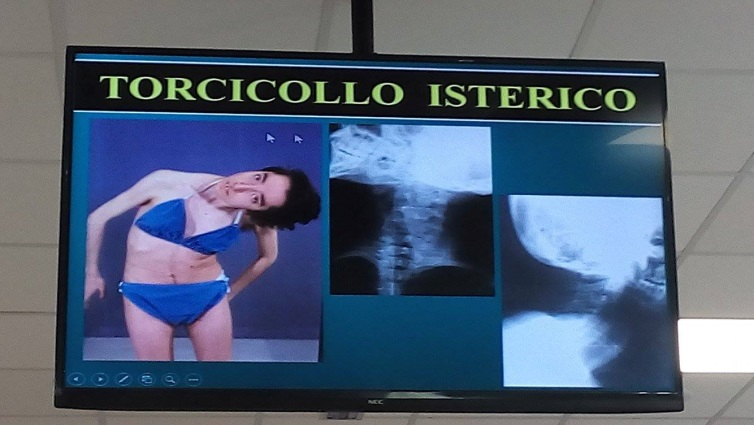
\includegraphics[width=0.4\textwidth]{013/image33.jpeg}
\end{figure}

L'isteria può mimare tante patologie. Non c'è nulla di organico. Vanno trattati con Valium.

\subsubsection{Torcicollo oculare}

\begin{figure}[!ht]
\centering
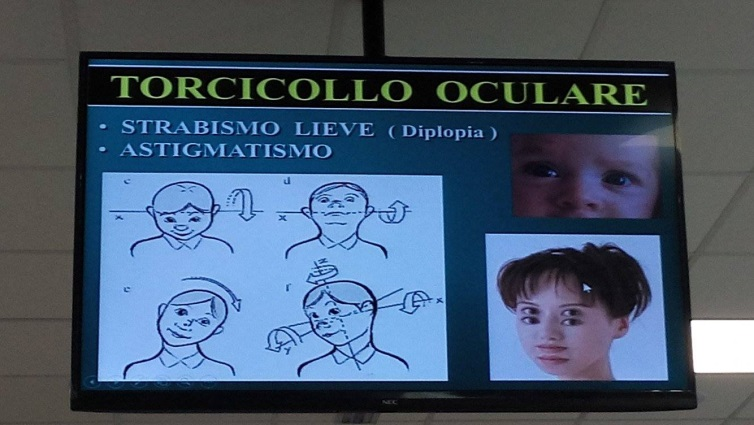
\includegraphics[width=0.4\textwidth]{013/image34.jpeg}
\end{figure}

Lo \textbf{strabismo lieve} dà una \emph{diplopia} quindi per sovrapporre l'immagine il paziente piega il capo e questo porta il bambino a inclinare la testa per sovrapporre i margini della visione.

Lo \textbf{strabismo grave} invece porta a \emph{esclusione di un occhio} dalla visione da parte del cervello quindi non elabora le informazioni visive.

In questi casi si chiude l'occhio e si vede se il torcicollo migliora.
Il torcicollo oculare scompare correggendo il difetto oculare.

\subsubsection{Torcicollo otogeno}

Le otiti purulente e le mastoiditi danno grosso dolore che può portare ad un atteggiamento antalgico che simula un torcicollo

\subsubsection{Torcicollo miopatico}

\begin{figure}[!ht]
\centering
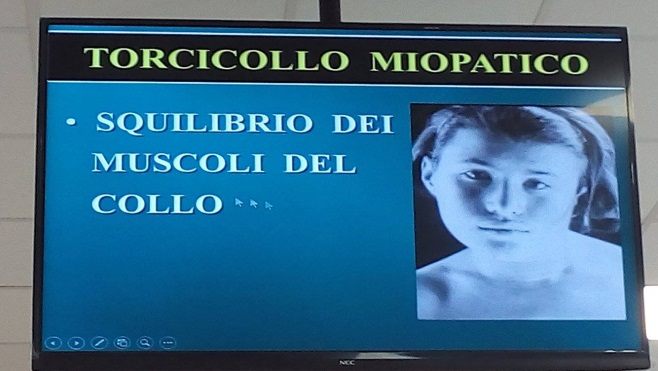
\includegraphics[width=0.4\textwidth]{013/image35.jpeg}
\end{figure}

\emph{Le miopatie possono causare con un'alterazione dell'equilibrio (squilibri) dei due sternocleidomastoidei.}
